\documentclass[xcolor=dvipsnames,10pt]{beamer}
\mode<presentation>


\usepackage[active,tightpage]{preview}
%\setlength\PreviewBorder{5pt}%
%\usepackage[hidelinks]{hyperref}
%\usepackage{cite}
\usepackage{beamerthemesplit}
\usepackage{verbatim}
\usepackage[UKenglish]{babel}
\usepackage{listings}
\usepackage{latexsym}
\usepackage[utf8]{inputenc}
\usepackage{multirow}
\usepackage{listings}
\usepackage{color}
\usepackage{amsmath,amsthm,amssymb}
\usepackage[noend]{algpseudocode}
\usepackage[ruled,noline,linesnumbered]{algorithm2e}
\usepackage{pgf}
\usepackage{tikz}
\usetikzlibrary{automata,arrows,decorations.pathreplacing}
	\usetikzlibrary{positioning}
	\usetikzlibrary{backgrounds}
	\usetikzlibrary{arrows}
\usepackage{epstopdf}
\usepackage[caption=false]{subfig}

\usepackage{array}
\newcolumntype{C}[1]{>{\centering\arraybackslash}p{#1}}


%% style for drawing RNNs
\tikzstyle{RNN_style}=[
	->,shorten >=1pt,auto,node distance=1.5cm, thick,
	neuron/.style={circle,fill=white!50,node distance =1.2cm,draw,minimum 	size=0.7cm,font=\sffamily\normalsize},
	missing/.style={rectangle,node distance =1.2cm,draw=none,minimum size=0.7cm,font=\sffamily\Huge\bfseries},
	label/.style={node distance=1.2cm,rectangle,draw=none,minimum size=0.7cm,font=\sffamily\normalsize},
	layer/.style={rectangle,fill=white!50,draw,minimum width=4cm,font=\sffamily\normalsize},
	thick_edge/.style={line width=1pt},
	thin_edge/.style={line width=0.5pt}
]

%%Notation:

%%vectors
\renewcommand{\vec}[1]{\boldsymbol{#1}}
%%sets
\newcommand{\set}[1]{\mathcal{#1}}
%%matrixes
\newcommand{\mat}[1]{#1}
%%norm
\newcommand{\norm}[1]{\left\Vert #1 \right\Vert}
%%defeq
\newcommand{\defeq}{\triangleq}
%%
\newcommand{\net}[1]{\mathrm{#1}}
%% pair<x,y>
\newcommand{\pair}[2]{\langle#1,#2\rangle}


\graphicspath{ {./images/} }

%\usecolortheme[named=MidnightBlue]{structure}
%Warsaw Dresden Singapore Copenhagen Madrid AnnArbor
%\usetheme{Warsaw}
\usetheme{metropolis}
\setbeamercovered{transparent}
%\setbeamercolor{lowercolor}{fg=white , bg=MidnightBlue}
\setbeamertemplate{blocks}[rounded][shadow=true]
\setbeamertemplate{items}[default]
\setbeamertemplate{navigation symbols}{}

\title{Optimization methods for Recurrent Neural Networks training}
%\subtitle{A nice subtitle}
\date{20th April 2016}
\author{Giulio Galvan\\ Gsss }
\institute{Università degli studi di Firenze}
\titlegraphic{\hfill\includegraphics[height=1.5cm]{stemma}}  % %TODO put the logo img here
\usetitlepagetemplate{
	\begin{center}
		%\pgfuseimage{salom}
		%\vskip0.5ex
		\begin{figure}
			\includegraphics[width=3cm]{stemma.pdf}
		\end{figure}
		\vskip4ex
		\begin{beamerboxesrounded}[lower=lowercolor, shadow=true]{}
			\begin{center}
				\large{\textbf{Optimization methods for Recurrent Neural Networks training}}\\
				
			\end{center}
		\end{beamerboxesrounded}
		\vskip4ex
		\begin{footnotesize}
			\begin{center}
				Giulio Galvan
			\end{center}
			\begin{columns}
				\begin{column}{0.4\textwidth}
					\flushleft{\textbf{Relatori}: }\\
					Prof. Marco Sciandrone \\
					Prof. Luís  Nunes Vicente
				\end{column}
				\begin{column}{0.4\textwidth}
					\flushright{\textbf{Correlatore}: }\\
					Prof. Fabio Schoen
				\end{column}
			\end{columns}
			\vskip 1cm
			20th April 2016
		\end{footnotesize}
		
	\end{center}
}


\begin{document}
%\maketitle
\frame{\titlepage}
\section{Introduction}
 
\begin{frame}{The model}
	
\begin{block}{RNN}
	Given an input sequences $\{\vec{u}\}_{t=1,...,T}$, with $ \vec{u}_t \in \mathbb{R}^p$, the output sequence of a RNN $\{\vec{y}\}_{t=1,...,T}$, with $\vec{y}_t \in \mathbb{R}^o$,  is defined by the following:
\begin{align}
		&\vec{y}^t \defeq F(W^{out}\cdot\vec{a}^t + \vec{b}^{out})\\
		&\vec{a}^t \defeq W^{rec}\cdot\vec{h}^{t-1}+W^{in}\cdot\vec{u}^t+\vec{b}^{rec}\\
		&\vec{h}^t \defeq  \sigma(\vec{a}^t) \\
		&\vec{h}^0 \defeq \overrightarrow{0},
\end{align}
where $\sigma(\cdot):\mathbb{R}\rightarrow\mathbb{R}$ is a non linear function applied element-wise called activation function.
\end{block}
\end{frame}

\begin{frame}{The optimization problem}
Given a dataset $D$:
\begin{equation}
D\defeq\{\{\overline{\vec{u}}^{(i)}\}_{t=1,...,T}, \overline{\vec{u}}^{(i)}_t \in \mathbb{R}^p, \{\overline{\vec{y}}^{(i)}\}_{t=1,...,T}, \overline{\vec{y}}^{(i)}_t \in \mathbb{R}^o;  i=1,...,N\}
\end{equation}
we define a loss function $L_D:\mathbb{R}^N \rightarrow \mathbb{R}_{\geq 0}$ over $D$  as
\begin{equation}
L_D(\vec{x})\defeq\frac{1}{N}\sum_{i=1}^N \sum_{t=1}^T L_t(\overline{\vec{y}}_t^{(i)},\vec{y}_t^{(i)}(\vec{x})),
\end{equation}
where $L_t(\cdot, \cdot)$ is an arbitrary loss function for the time step $t$.
The problem is \begin{equation}
\min_{\vec{x}\in \mathbb{R}^N} L_D(\vec{x})
\end{equation}
\end{frame}

\begin{frame}{Stochastic gradient descent (SGD)}
SGD is the standard framework in most of the applications.
\begin{algorithm}[H]
	\KwData{\\
		\Indp
		$D=\{\pair{\vec{u}^{(i)}}{\vec{y}^{(i)}}\}$: training set\\
		$\vec{x}_0$: candidate solution \\
		$m$: size of each minibatch\\
	}
	
	\KwResult{\\
		\Indp $\vec{x}$: solution
	}
	\BlankLine
	
	$\vec{x} \gets \vec{x}_0$\\
	\While{stop criterion}{
		
		$I$ $\gets$ select $m$ training example $\in D$  \\
		$\alpha \gets$ compute learning rate \\
		$\vec{x} \gets \vec{x} - \alpha \sum_{ i\in I}\nabla_{\vec{x}} L(\vec{x}; \pair{\vec{u}^{(i)}}{\vec{y}^{(i)}})$\\
	}
	\caption{Stochastic gradient descent}
	\label{algo:sgd}
\end{algorithm}	
\end{frame}
\section{Gradient of a RNN}
\documentclass{article}
\usepackage[utf8]{inputenc}
\usepackage[italian]{babel}
\usepackage{graphicx}
\usepackage{cite}
\usepackage[hidelinks]{hyperref}
\usepackage{listings}
\usepackage{latexsym}
\usepackage{amsmath}
\usepackage{proof}
\usepackage{stmaryrd}
\usepackage{amssymb}
\usepackage{epstopdf}
\usepackage{pgf}
\usepackage{tikz}
\usepackage{algorithm}
\usepackage[noend]{algpseudocode}
\usetikzlibrary{automata,arrows}
\let\emptyset\varnothing

\graphicspath{ {./images/} }

\title{On Gradient}
\author{Giulio Galvan}

\begin{document}
\maketitle

\begin{abstract}
\end{abstract}

\section{How to compute gradient}
\subsection{Backpropagation}

First of all we need to define a loss function over the training data, so we define a dataset as 

\begin{equation}
D=\{x^{(i)} \in \mathbb{R}^p, y^{(i)} \in \mathbb{R}^q,  i\in[1,N]\}
\end{equation}

and the loss function as
\begin{equation}
L(W)=\frac{1}{N}\sum_{i=1}^N L^{(i)}(W) 
\end{equation}

where $W$ is represents all the weights of the net.
The network is defined by
\begin{equation}
a_l = \sum_j w_{lj}\phi_j
\end{equation}

\begin{equation}
\phi_l = \sigma(a_l)
\end{equation}


where $w_{lj}$ is the weight of the connection between neuron $j$ and neuron $l$ and $\sigma$ is the non linear activation function

So we can compute partial derivatives with respect to a single weight $w_{lj}$, using simply the chain ruly, as 

$$\frac{\partial L^{(i)}}{\partial w_{lj}}=\frac{\partial L^{(i)}}{\partial a_l} \cdot \frac{\partial a_l}{\partial w_{lj}}=\delta_l \cdot \phi_j$$
where we put 
$$\delta_l \triangleq \frac{\partial L^{(i)}}{\partial a_l}$$


So we can easily compute $\delta_u = \frac{\partial L^{(i)}}{\partial a_u} $ for each output unit $u$ once we choose a differtiable loss function; note
that we dont need the weights for such a computation. 

Let $P(l)$ be the set of parents of neuron $l$, formally:
\begin{equation} 
P(l) = \{ k: \exists \text{ a link between $l$ and $k$ with weight } w_{lk} \}
\end{equation}

Again, simply using the chain rule, we can write:

$$\delta_l = \sum_{k\in P(l)} \frac{\partial L^{(i)}}{\partial a_k} \cdot \frac{\partial a_k}{\partial a_l}= \sum_{k\in P(l)} \delta_k \cdot 
\frac{\partial a_k}{\partial \phi_l} \cdot \frac{\partial \phi_l}{\partial a_l} = \sum_{k\in P(l)} \delta_k \cdot 
w_{kl} \cdot \sigma'(a_l) $$



\newpage
\nocite{*}		 % Mostra in bibliografia anche gli oggetti non citati 
\bibliography{biblio}{}
\bibliographystyle{plain}


\end{document}     
\section{The vanishing gradient problem}
\begin{frame}{A pathological problem example}


An input sequence:

\vspace{1em}

\begin{tabular}{|c|c|c|c|c|c|c|c|c|c}
	\hline  marker & 0&  1&  0&  $\hdots$& 0 & 1 & 0 & 0  \\ 
	  value & 0.3&  \textbf{0.7}&  0.1&  $\hdots$& 0.2& \textbf{0.4} & 0.6& 0.9  \\ 
	\hline 
\end{tabular}

\vspace{1em}
The predicted output should be the sum of the two one marked positions (1.1). 
\pause
\vspace{1em}
\begin{block}{Why is this a difficult problem?}
	\pause
	Because of it's long time dependencies.
\end{block}

\end{frame}

\begin{frame}{Unfolding}
	\tikzstyle{rnn_style}=[->,shorten >=1pt,auto,node distance=1.5cm,
	thick,
	neuron/.style={circle,fill=white!50,draw,minimum size=0.7cm,font=\sffamily\Large\bfseries},
	missing/.style={circle,fill=white!50,draw=none,minimum size=0.7cm,font=\sffamily\Huge\bfseries},
	label/.style={node distance=1.2cm,rectangle,fill=white!50,draw=none,minimum size=0.7cm,font=\sffamily\normalsize},
	layer/.style={rectangle,fill=white!50,draw,minimum width=4cm,font=\sffamily\normalsize},
	loopStyle/.style={in=120,out=60, distance=2.5cm},]
	

		
	\begin{figure}[h!]
		\centering
		\resizebox{8cm}{!}{
		\begin{tikzpicture}[rnn_style]
		
		%t=0
		\node[layer] (hl1) {Hidden layer t=0};
		
		\node[neuron]    (x0)[below left=0.3cm and 1cm of hl1]       {};
		\node[label]    (u0)[left of=x0]   {$\vec{u}_1$};
		
		
		
		\node[neuron] (o0) [above right=0.3cm and 1cm of hl1] {};
		\node[label]    (y0)[right of=o0]   {$\vec{y}_1$};
		
		%t=1
		\node[layer] (hl2)[above of=hl1,node distance=2.5cm] {Hidden layer t=1};
		
		\node[neuron]    (x1)[below left=0.3cm and 1cm of hl2]      {};
		\node[label]    (u1)[left of=x1]   {$\vec{u}_2$};
		
		
		\node[neuron] (o1) [above right=0.3cm and 1cm of hl2] {};
		\node[label]    (y1)[right of=o1]   {$\vec{y}_2$};
		
		%dots
		\node[label,font=\sffamily\Huge\bfseries] (hld)[above of=hl2,node distance=2cm] {$\hdots$};
		
		%t=T
		\node[layer] (hlT)[above of=hld,node distance=2cm] {Hidden layer t=T};
		
		\node[neuron]    (xT)[below left=0.3cm and 1cm of hlT]      {};
		\node[label]    (uT)[left of=xT]   {$\vec{u}_T$};
		
		
		\node[neuron] (oT) [above right=0.3cm and 1cm of  hlT] {};
		\node[label]    (yT)[right of=oT]   {$\vec{y}_T$};
		
		
		%biases
		\node[neuron](b) [right of=y1,node distance=1.4cm] {};
		\node[label] (b_l) [above of=b,node distance=0.7cm] {bias=1};
		
		
		\path[->] (x0) edge [bend right] node[]{$W^{in}$}   (hl1)
		(u0) edge []   (x0)
		(o0) edge []   (y0)
		(x1) edge [bend right] node[]{$W^{in}$} (hl2)
		(u1) edge []   (x1)
		(o1) edge []   (y1)
		(xT) edge [bend right] node[]{$W^{in}$} (hlT)
		(uT) edge []   (xT)
		(oT) edge []   (yT)
		
		
		(hl1) edge [bend left]  node[]{$W^{out}$} (o0)
		(hl2) edge [bend left]  node[]{$W^{out}$} (o1)
		(hlT) edge [bend left]  node[]{$W^{out}$} (oT)
		
		(b)  edge [bend left,dotted,in = 90]  node[]{$b^{out}$} (o0)
		(b)  edge [bend left, dotted, in = 90,out=80]  node[]{$b^{rec}$} (hl1)
		(b)  edge [bend left, dotted]  node[]{$b^{rec}$} (hl2)
		(b)  edge [bend left,dotted]  node[]{$b^{out}$} (o1)
		(b)  edge [bend left, dotted,in = 200]  node[]{$b^{rec}$} (hlT)
		(b)  edge [bend left,dotted,in =200]  node[]{$b^{out}$} (oT)
		(hl1) edge [] node[]{$W^{rec} $} (hl2)
		(hl2) edge [] node[]{$W^{rec} $} (hld)
		(hld) edge [] node[]{$W^{rec} $} (hlT);
		
		\end{tikzpicture}
	}
		\caption{Unfolding of a $\net{RNN}$}
		\label{rnn_unfolding}
	\end{figure}
\end{frame}

\begin{frame}{Understanding the gradient structure}
	Simply applying the chain rule it's easy to see that
	\begin{equation}
		\nabla L(\vec{x}) = \sum_{t=1}^T \nabla L_{|t}(\vec{x}),
	\end{equation}
	where $\nabla L_{|t}$ is ...
\end{frame}

\begin{frame}{Vanishing gradient: an upper bound}
	\begin{equation}
	\frac{\partial \vec{a}^t}{\partial \vec{a}^k} = \prod_{i=t-1}^{k}  diag(\sigma'(\vec{a}^i)) \cdot \mat{W}^{rec}.
	\label{eq:temporalComponent}
	\end{equation}
	
	Taking the singular value decomposition of $\mat{W}^{rec}$:
	\begin{equation}
	\mat{W}^{rec} =  \mat{S}\cdot\mat{D}\cdot\mat{V}^T
	\end{equation}
	where $\mat{S},\mat{V}^T$ are squared orthogonal matrices and $\mat{D}\defeq diag(\mu_1, \mu_2,...,\mu_r)$ is the diagonal matrix containing the singular values of $\mat{W}^{rec}$.
	Hence:
	\begin{equation}
	\frac{\partial \vec{a}^t}{\partial \vec{a}^k} = \prod_{i=t-1}^{k}  diag(\sigma'(\vec{a}^i)) \cdot \mat{S}\cdot \mat{D} \cdot \mat{V}^T
	\end{equation}
	\end{frame}
	\begin{frame}
			Since $\mat{U}$ and $\mat{V}$ are orthogonal matrix, hence $$\norm{\mat{U}}_2=\norm{\mat{V}^T}_2 = 1,$$ and $$\norm{diag(\lambda_1, \lambda_2,...,\lambda_r)}_2 \leq \lambda_{max},$$ we get
			\begin{align}
			\norm{\frac{\partial \vec{a}^t}{\partial \vec{a}^k}}_2 &= \norm{ (\prod_{i=t-1}^{k} diag(\sigma'(\vec{a}^i)) \cdot \mat{S}\cdot \mat{D} \cdot \mat{V}^T)}_2\\
			&\leq (\sigma'_{max} \cdot \mu_{max})^{t-k-1}
			\end{align}
	\end{frame}



\begin{frame}{Temporal gradient norms: an illustration}
\begin{figure}
	\centering
	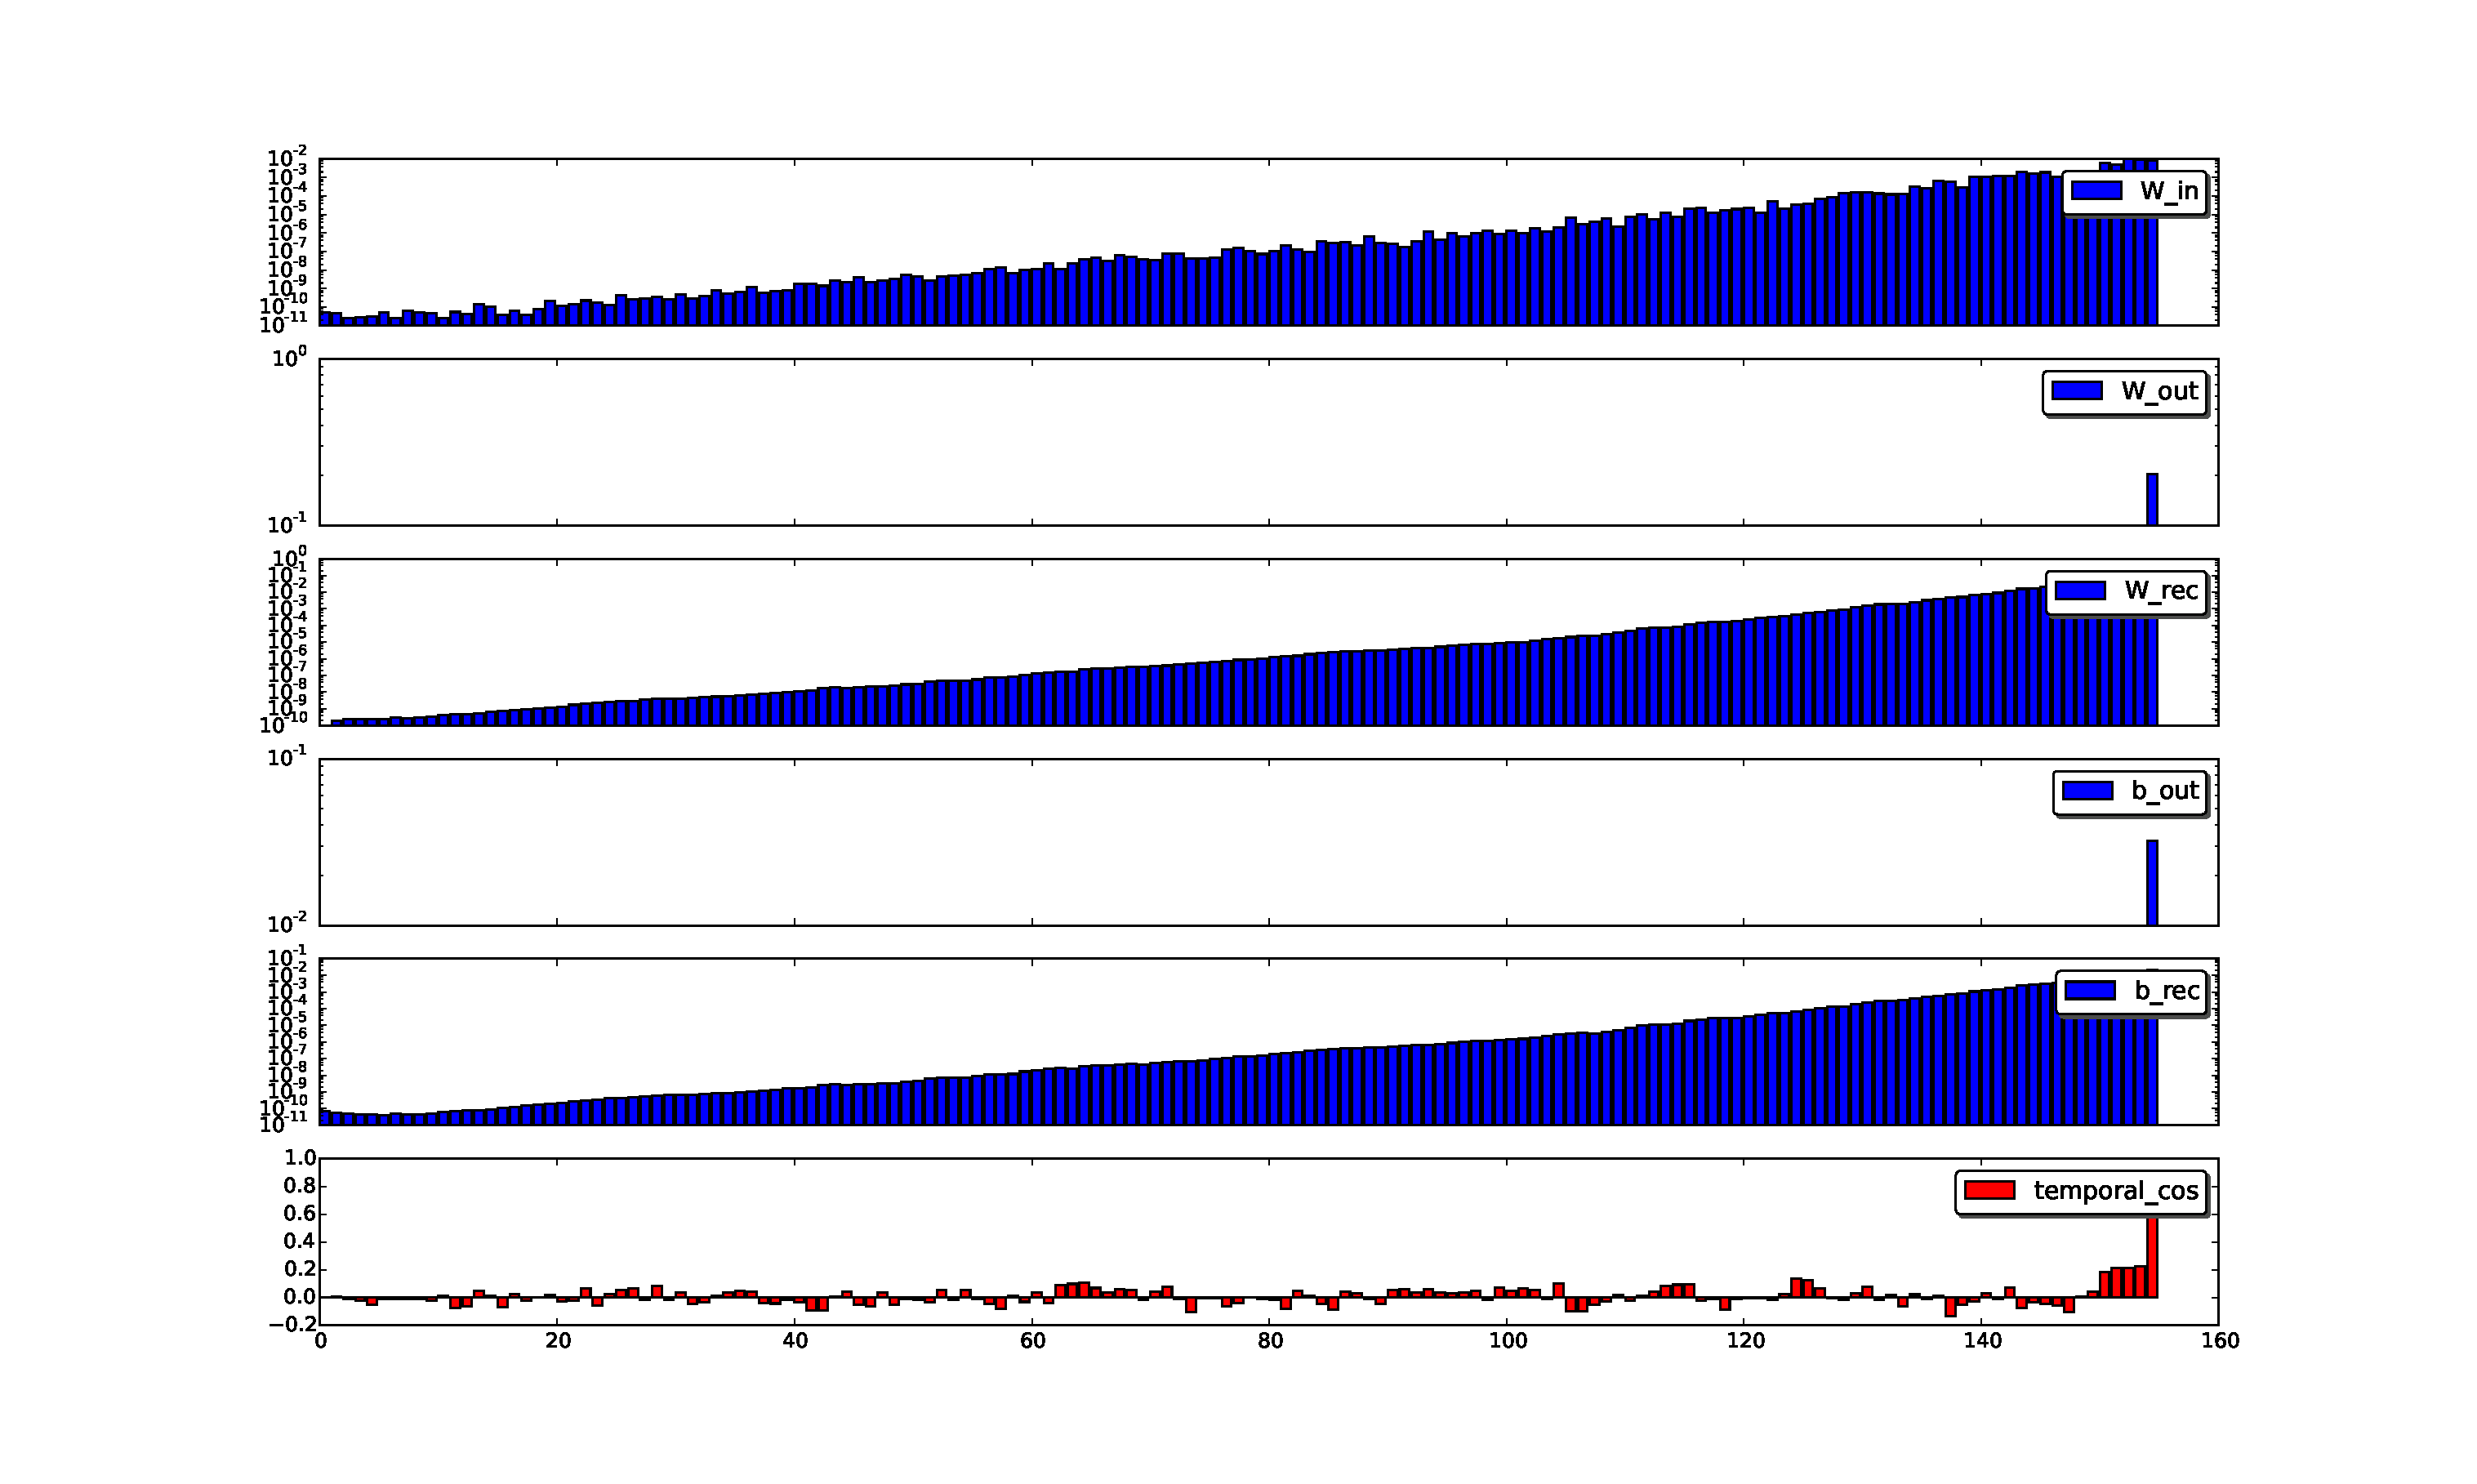
\includegraphics[width=1\textwidth]{temporal_gradients.eps}
\end{figure}
\end{frame}


%\section{Existing solutions}
%\begin{frame}{Existent solutions}
	
	\pause
	\begin{itemize}
		\item Long short-term memory (LSTM). Hochreiter, Schmidhuber (1997)
			\begin{itemize}
				\item the network structure is modified with specialized "memory cells"
				\item a truncated version of back-propagation is employed
			\end{itemize}
		\pause
		\item Hessian-Free optimization (HF). Martens (2010)
		\begin{itemize}
			\item a second order method
			\item a "cheap" approximation of the Hessian is employed
			\item the quadratic sub-problem is solved through conjugate gradient + structural damping
		\end{itemize}
		\pause
		\item Pascanu, Bengio (2013)
		\begin{itemize}
			\item a first order method
			\item uses a penalty to deal with the vanishing gradient problem
		\end{itemize}
	\end{itemize}
	
\end{frame}

\begin{frame}{A new proposal}
\begin{itemize}
	\item use the structure of the gradient to compute a descent direction which does not suffer from the vanishing gradient problem
	
	\item normalize the temporal components
	\begin{equation}
	d(\vec{x}) = \sum_{t=1}^T \frac{\nabla L_{|t}(\vec{x})}{\norm{\nabla L_{|t}(\vec{x})}}
	\end{equation}
	
	\item add some randomness for robustness:
		\begin{equation}
		d(\vec{x}) = \sum_{t=1}^T \beta_t\frac{\nabla L_{|t}(\vec{x})}{\norm{\nabla L_{|t}(\vec{x})}},
		\end{equation}
		
		with $\sum_{t=1}^T\beta_t=1, \beta_t>0$
\end{itemize}



\end{frame}

\section{A new SGD approach for training RNNs}
\begin{frame}{Initialization}
	
The matrix $\mat{W}^{rec}$ is \textbf{scaled} to have a desired spectral radius.

\vspace{2em}

\begin{algorithm}[H]
	\KwData{\\
		\Indp
		$\rho = $ desired spectral radius
	}
	\BlankLine
	
	$\mat{W_{rec}} \sim \mathcal{N}(0, \sigma^2)$\\
	$r \gets \mbox{spectral\_radius}(\mat{W_{rec}})$\\
	$\mat{W_{rec}}\gets \frac{\rho}{r} \cdot \mat{W_{rec}}$\\
	\KwRet{$\mat{W_{rec}}$}
	\caption{Recurrent weight matrix initialization scheme}
	\label{algo:init_scaling}
\end{algorithm}
\end{frame}

\begin{frame}{The effect of initialization on the temporal gradients}
	\captionsetup[subfigure]{labelformat=empty}
		\begin{figure}
			\centering
			\subfloat[][]{\includegraphics[width= 0.5\textwidth]{plot_grad_norms_it0_09.eps}\label{fig:temp_norms_09}}
			\subfloat[][]{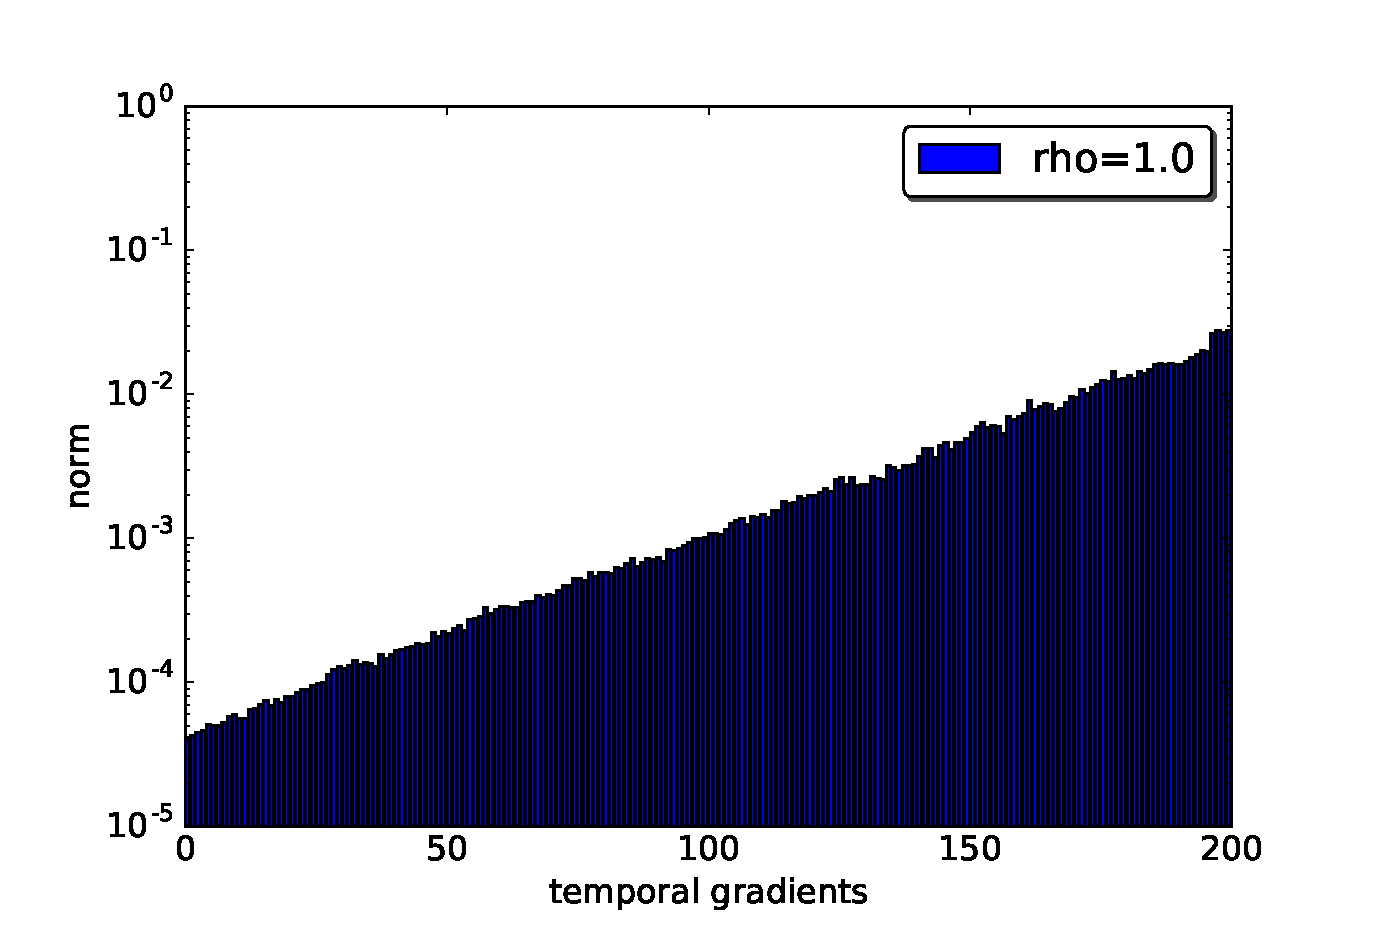
\includegraphics[width= 0.5\textwidth]{plot_grad_norms_it0_1.eps}\label{fig:temp_norms_1}}\\
			\vspace{-2em}
			\subfloat[][]{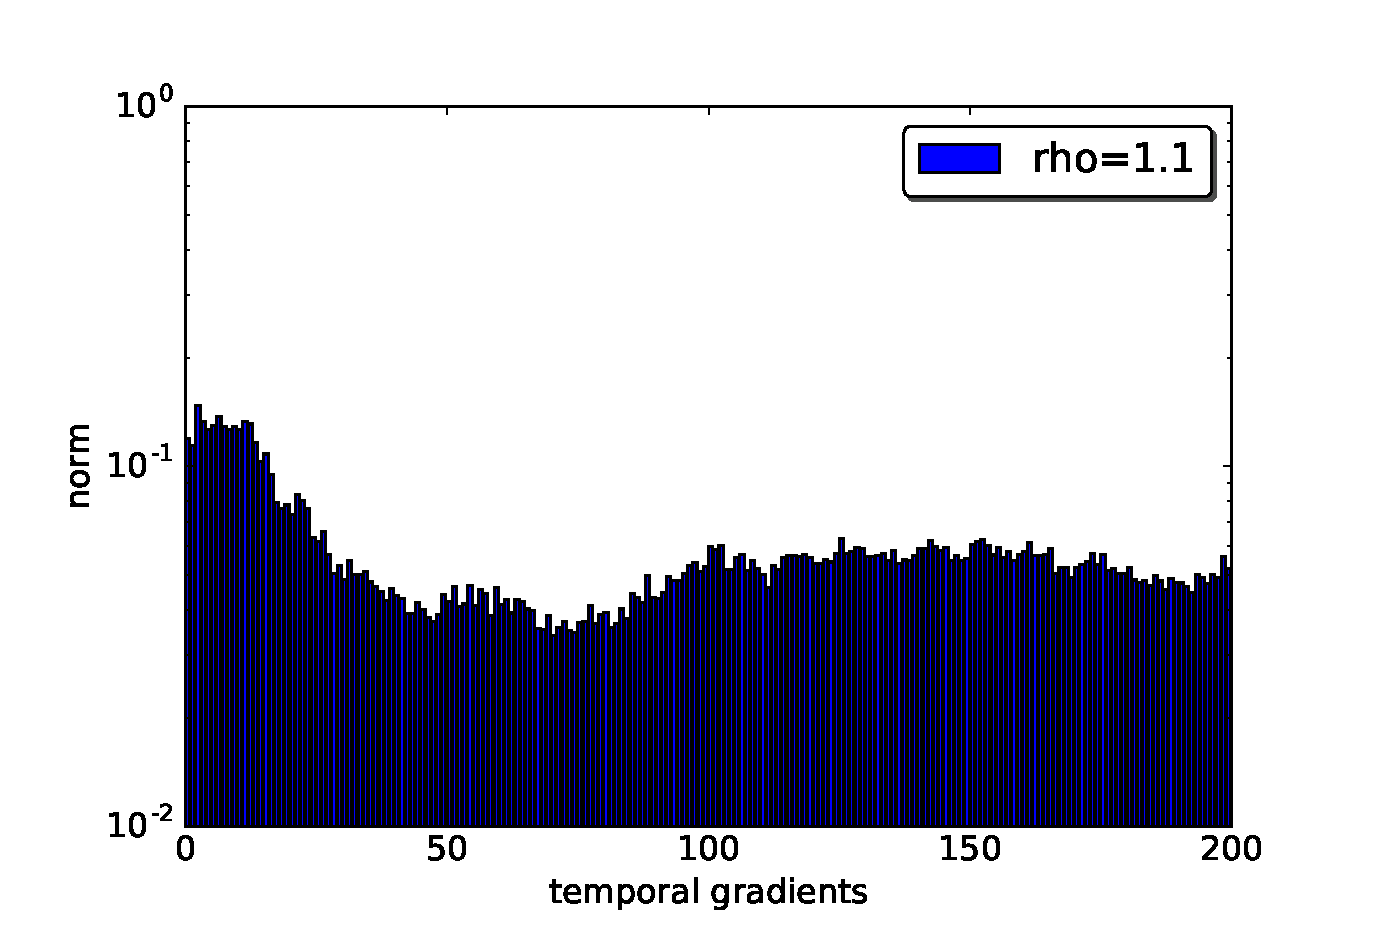
\includegraphics[width= 0.5\textwidth]{plot_grad_norms_it0_11.eps}\label{fig:temp_norms_11}}
			\subfloat[][]{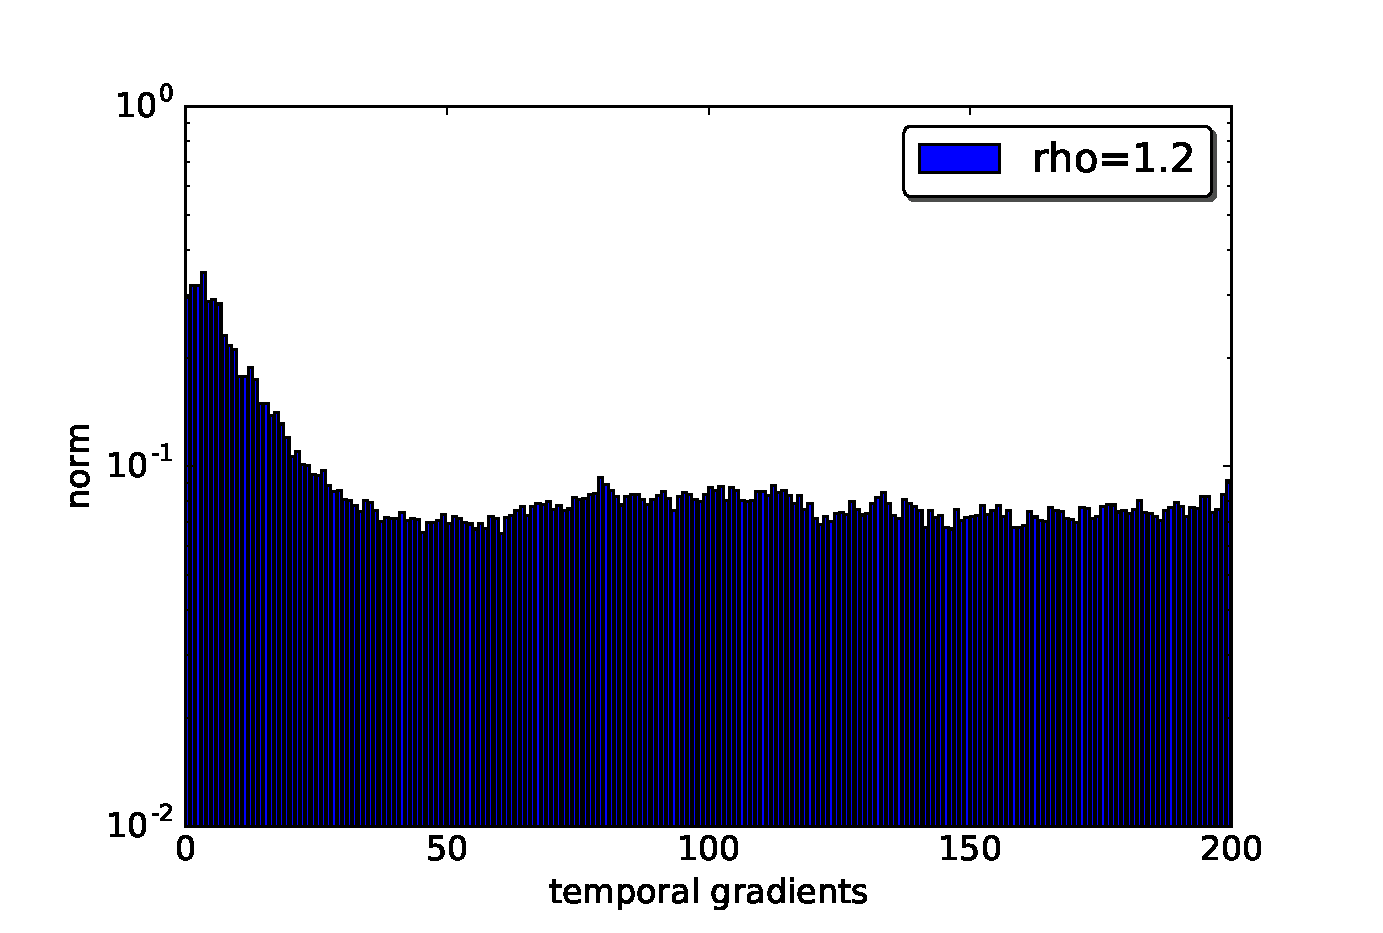
\includegraphics[width= 0.5\textwidth]{plot_grad_norms_it0_12.eps}\label{fig:temp_norms_12}}
		\end{figure}
	
%	\vspace{-3em}
%	\begin{figure}[H]
%		\includegraphics[width=0.6\textwidth]{temporal_components_rho.eps}
%		\caption{Temporal gradients for the temporal order task varying the spectral radius of the recurrent matrix. y axis is in logarithmic scale.}
%		\label{fig:temporal_norms}
%	\end{figure}
\end{frame}

\begin{frame}{The effect of initialization on the rate of success}
	\begin{figure}
		\centering
%		%% Creator: Matplotlib, PGF backend
%%
%% To include the figure in your LaTeX document, write
%%   \input{<filename>.pgf}
%%
%% Make sure the required packages are loaded in your preamble
%%   \usepackage{pgf}
%%
%% Figures using additional raster images can only be included by \input if
%% they are in the same directory as the main LaTeX file. For loading figures
%% from other directories you can use the `import` package
%%   \usepackage{import}
%% and then include the figures with
%%   \import{<path to file>}{<filename>.pgf}
%%
%% Matplotlib used the following preamble
%%   \usepackage{fontspec}
%%   \setmainfont{DejaVu Serif}
%%   \setsansfont{DejaVu Sans}
%%   \setmonofont{DejaVu Sans Mono}
%%
\begingroup%
\makeatletter%
\begin{pgfpicture}%
\pgfpathrectangle{\pgfpointorigin}{\pgfqpoint{8.000000in}{6.000000in}}%
\pgfusepath{use as bounding box, clip}%
\begin{pgfscope}%
\pgfsetbuttcap%
\pgfsetmiterjoin%
\definecolor{currentfill}{rgb}{1.000000,1.000000,1.000000}%
\pgfsetfillcolor{currentfill}%
\pgfsetlinewidth{0.000000pt}%
\definecolor{currentstroke}{rgb}{1.000000,1.000000,1.000000}%
\pgfsetstrokecolor{currentstroke}%
\pgfsetdash{}{0pt}%
\pgfpathmoveto{\pgfqpoint{0.000000in}{0.000000in}}%
\pgfpathlineto{\pgfqpoint{8.000000in}{0.000000in}}%
\pgfpathlineto{\pgfqpoint{8.000000in}{6.000000in}}%
\pgfpathlineto{\pgfqpoint{0.000000in}{6.000000in}}%
\pgfpathclose%
\pgfusepath{fill}%
\end{pgfscope}%
\begin{pgfscope}%
\pgfsetbuttcap%
\pgfsetmiterjoin%
\definecolor{currentfill}{rgb}{1.000000,1.000000,1.000000}%
\pgfsetfillcolor{currentfill}%
\pgfsetlinewidth{0.000000pt}%
\definecolor{currentstroke}{rgb}{0.000000,0.000000,0.000000}%
\pgfsetstrokecolor{currentstroke}%
\pgfsetstrokeopacity{0.000000}%
\pgfsetdash{}{0pt}%
\pgfpathmoveto{\pgfqpoint{1.000000in}{0.600000in}}%
\pgfpathlineto{\pgfqpoint{7.200000in}{0.600000in}}%
\pgfpathlineto{\pgfqpoint{7.200000in}{5.400000in}}%
\pgfpathlineto{\pgfqpoint{1.000000in}{5.400000in}}%
\pgfpathclose%
\pgfusepath{fill}%
\end{pgfscope}%
\begin{pgfscope}%
\pgfpathrectangle{\pgfqpoint{1.000000in}{0.600000in}}{\pgfqpoint{6.200000in}{4.800000in}} %
\pgfusepath{clip}%
\pgfsetbuttcap%
\pgfsetroundjoin%
\pgfsetlinewidth{1.003750pt}%
\definecolor{currentstroke}{rgb}{0.000000,0.000000,1.000000}%
\pgfsetstrokecolor{currentstroke}%
\pgfsetdash{{6.000000pt}{6.000000pt}}{0.000000pt}%
\pgfpathmoveto{\pgfqpoint{1.281818in}{5.000000in}}%
\pgfpathlineto{\pgfqpoint{1.563636in}{5.000000in}}%
\pgfpathlineto{\pgfqpoint{2.409091in}{5.000000in}}%
\pgfpathlineto{\pgfqpoint{3.818182in}{3.640000in}}%
\pgfpathlineto{\pgfqpoint{5.227273in}{3.640000in}}%
\pgfpathlineto{\pgfqpoint{6.636364in}{1.000000in}}%
\pgfusepath{stroke}%
\end{pgfscope}%
\begin{pgfscope}%
\pgfpathrectangle{\pgfqpoint{1.000000in}{0.600000in}}{\pgfqpoint{6.200000in}{4.800000in}} %
\pgfusepath{clip}%
\pgfsetbuttcap%
\pgfsetroundjoin%
\definecolor{currentfill}{rgb}{0.000000,0.000000,1.000000}%
\pgfsetfillcolor{currentfill}%
\pgfsetlinewidth{0.501875pt}%
\definecolor{currentstroke}{rgb}{0.000000,0.000000,0.000000}%
\pgfsetstrokecolor{currentstroke}%
\pgfsetdash{}{0pt}%
\pgfsys@defobject{currentmarker}{\pgfqpoint{-0.041667in}{-0.041667in}}{\pgfqpoint{0.041667in}{0.041667in}}{%
\pgfpathmoveto{\pgfqpoint{0.000000in}{-0.041667in}}%
\pgfpathcurveto{\pgfqpoint{0.011050in}{-0.041667in}}{\pgfqpoint{0.021649in}{-0.037276in}}{\pgfqpoint{0.029463in}{-0.029463in}}%
\pgfpathcurveto{\pgfqpoint{0.037276in}{-0.021649in}}{\pgfqpoint{0.041667in}{-0.011050in}}{\pgfqpoint{0.041667in}{0.000000in}}%
\pgfpathcurveto{\pgfqpoint{0.041667in}{0.011050in}}{\pgfqpoint{0.037276in}{0.021649in}}{\pgfqpoint{0.029463in}{0.029463in}}%
\pgfpathcurveto{\pgfqpoint{0.021649in}{0.037276in}}{\pgfqpoint{0.011050in}{0.041667in}}{\pgfqpoint{0.000000in}{0.041667in}}%
\pgfpathcurveto{\pgfqpoint{-0.011050in}{0.041667in}}{\pgfqpoint{-0.021649in}{0.037276in}}{\pgfqpoint{-0.029463in}{0.029463in}}%
\pgfpathcurveto{\pgfqpoint{-0.037276in}{0.021649in}}{\pgfqpoint{-0.041667in}{0.011050in}}{\pgfqpoint{-0.041667in}{0.000000in}}%
\pgfpathcurveto{\pgfqpoint{-0.041667in}{-0.011050in}}{\pgfqpoint{-0.037276in}{-0.021649in}}{\pgfqpoint{-0.029463in}{-0.029463in}}%
\pgfpathcurveto{\pgfqpoint{-0.021649in}{-0.037276in}}{\pgfqpoint{-0.011050in}{-0.041667in}}{\pgfqpoint{0.000000in}{-0.041667in}}%
\pgfpathclose%
\pgfusepath{stroke,fill}%
}%
\begin{pgfscope}%
\pgfsys@transformshift{1.281818in}{5.000000in}%
\pgfsys@useobject{currentmarker}{}%
\end{pgfscope}%
\begin{pgfscope}%
\pgfsys@transformshift{1.563636in}{5.000000in}%
\pgfsys@useobject{currentmarker}{}%
\end{pgfscope}%
\begin{pgfscope}%
\pgfsys@transformshift{2.409091in}{5.000000in}%
\pgfsys@useobject{currentmarker}{}%
\end{pgfscope}%
\begin{pgfscope}%
\pgfsys@transformshift{3.818182in}{3.640000in}%
\pgfsys@useobject{currentmarker}{}%
\end{pgfscope}%
\begin{pgfscope}%
\pgfsys@transformshift{5.227273in}{3.640000in}%
\pgfsys@useobject{currentmarker}{}%
\end{pgfscope}%
\begin{pgfscope}%
\pgfsys@transformshift{6.636364in}{1.000000in}%
\pgfsys@useobject{currentmarker}{}%
\end{pgfscope}%
\end{pgfscope}%
\begin{pgfscope}%
\pgfpathrectangle{\pgfqpoint{1.000000in}{0.600000in}}{\pgfqpoint{6.200000in}{4.800000in}} %
\pgfusepath{clip}%
\pgfsetbuttcap%
\pgfsetroundjoin%
\pgfsetlinewidth{1.003750pt}%
\definecolor{currentstroke}{rgb}{1.000000,0.000000,0.000000}%
\pgfsetstrokecolor{currentstroke}%
\pgfsetdash{{6.000000pt}{6.000000pt}}{0.000000pt}%
\pgfpathmoveto{\pgfqpoint{1.281818in}{5.000000in}}%
\pgfpathlineto{\pgfqpoint{1.563636in}{5.000000in}}%
\pgfpathlineto{\pgfqpoint{2.409091in}{1.000000in}}%
\pgfpathlineto{\pgfqpoint{3.818182in}{1.000000in}}%
\pgfpathlineto{\pgfqpoint{5.227273in}{1.000000in}}%
\pgfpathlineto{\pgfqpoint{6.636364in}{1.000000in}}%
\pgfusepath{stroke}%
\end{pgfscope}%
\begin{pgfscope}%
\pgfpathrectangle{\pgfqpoint{1.000000in}{0.600000in}}{\pgfqpoint{6.200000in}{4.800000in}} %
\pgfusepath{clip}%
\pgfsetbuttcap%
\pgfsetroundjoin%
\definecolor{currentfill}{rgb}{1.000000,0.000000,0.000000}%
\pgfsetfillcolor{currentfill}%
\pgfsetlinewidth{0.501875pt}%
\definecolor{currentstroke}{rgb}{0.000000,0.000000,0.000000}%
\pgfsetstrokecolor{currentstroke}%
\pgfsetdash{}{0pt}%
\pgfsys@defobject{currentmarker}{\pgfqpoint{-0.041667in}{-0.041667in}}{\pgfqpoint{0.041667in}{0.041667in}}{%
\pgfpathmoveto{\pgfqpoint{0.000000in}{-0.041667in}}%
\pgfpathcurveto{\pgfqpoint{0.011050in}{-0.041667in}}{\pgfqpoint{0.021649in}{-0.037276in}}{\pgfqpoint{0.029463in}{-0.029463in}}%
\pgfpathcurveto{\pgfqpoint{0.037276in}{-0.021649in}}{\pgfqpoint{0.041667in}{-0.011050in}}{\pgfqpoint{0.041667in}{0.000000in}}%
\pgfpathcurveto{\pgfqpoint{0.041667in}{0.011050in}}{\pgfqpoint{0.037276in}{0.021649in}}{\pgfqpoint{0.029463in}{0.029463in}}%
\pgfpathcurveto{\pgfqpoint{0.021649in}{0.037276in}}{\pgfqpoint{0.011050in}{0.041667in}}{\pgfqpoint{0.000000in}{0.041667in}}%
\pgfpathcurveto{\pgfqpoint{-0.011050in}{0.041667in}}{\pgfqpoint{-0.021649in}{0.037276in}}{\pgfqpoint{-0.029463in}{0.029463in}}%
\pgfpathcurveto{\pgfqpoint{-0.037276in}{0.021649in}}{\pgfqpoint{-0.041667in}{0.011050in}}{\pgfqpoint{-0.041667in}{0.000000in}}%
\pgfpathcurveto{\pgfqpoint{-0.041667in}{-0.011050in}}{\pgfqpoint{-0.037276in}{-0.021649in}}{\pgfqpoint{-0.029463in}{-0.029463in}}%
\pgfpathcurveto{\pgfqpoint{-0.021649in}{-0.037276in}}{\pgfqpoint{-0.011050in}{-0.041667in}}{\pgfqpoint{0.000000in}{-0.041667in}}%
\pgfpathclose%
\pgfusepath{stroke,fill}%
}%
\begin{pgfscope}%
\pgfsys@transformshift{1.281818in}{5.000000in}%
\pgfsys@useobject{currentmarker}{}%
\end{pgfscope}%
\begin{pgfscope}%
\pgfsys@transformshift{1.563636in}{5.000000in}%
\pgfsys@useobject{currentmarker}{}%
\end{pgfscope}%
\begin{pgfscope}%
\pgfsys@transformshift{2.409091in}{1.000000in}%
\pgfsys@useobject{currentmarker}{}%
\end{pgfscope}%
\begin{pgfscope}%
\pgfsys@transformshift{3.818182in}{1.000000in}%
\pgfsys@useobject{currentmarker}{}%
\end{pgfscope}%
\begin{pgfscope}%
\pgfsys@transformshift{5.227273in}{1.000000in}%
\pgfsys@useobject{currentmarker}{}%
\end{pgfscope}%
\begin{pgfscope}%
\pgfsys@transformshift{6.636364in}{1.000000in}%
\pgfsys@useobject{currentmarker}{}%
\end{pgfscope}%
\end{pgfscope}%
\begin{pgfscope}%
\pgfsetrectcap%
\pgfsetmiterjoin%
\pgfsetlinewidth{1.003750pt}%
\definecolor{currentstroke}{rgb}{0.000000,0.000000,0.000000}%
\pgfsetstrokecolor{currentstroke}%
\pgfsetdash{}{0pt}%
\pgfpathmoveto{\pgfqpoint{7.200000in}{0.600000in}}%
\pgfpathlineto{\pgfqpoint{7.200000in}{5.400000in}}%
\pgfusepath{stroke}%
\end{pgfscope}%
\begin{pgfscope}%
\pgfsetrectcap%
\pgfsetmiterjoin%
\pgfsetlinewidth{1.003750pt}%
\definecolor{currentstroke}{rgb}{0.000000,0.000000,0.000000}%
\pgfsetstrokecolor{currentstroke}%
\pgfsetdash{}{0pt}%
\pgfpathmoveto{\pgfqpoint{1.000000in}{5.400000in}}%
\pgfpathlineto{\pgfqpoint{7.200000in}{5.400000in}}%
\pgfusepath{stroke}%
\end{pgfscope}%
\begin{pgfscope}%
\pgfsetrectcap%
\pgfsetmiterjoin%
\pgfsetlinewidth{1.003750pt}%
\definecolor{currentstroke}{rgb}{0.000000,0.000000,0.000000}%
\pgfsetstrokecolor{currentstroke}%
\pgfsetdash{}{0pt}%
\pgfpathmoveto{\pgfqpoint{1.000000in}{0.600000in}}%
\pgfpathlineto{\pgfqpoint{7.200000in}{0.600000in}}%
\pgfusepath{stroke}%
\end{pgfscope}%
\begin{pgfscope}%
\pgfsetrectcap%
\pgfsetmiterjoin%
\pgfsetlinewidth{1.003750pt}%
\definecolor{currentstroke}{rgb}{0.000000,0.000000,0.000000}%
\pgfsetstrokecolor{currentstroke}%
\pgfsetdash{}{0pt}%
\pgfpathmoveto{\pgfqpoint{1.000000in}{0.600000in}}%
\pgfpathlineto{\pgfqpoint{1.000000in}{5.400000in}}%
\pgfusepath{stroke}%
\end{pgfscope}%
\begin{pgfscope}%
\pgfsetbuttcap%
\pgfsetroundjoin%
\definecolor{currentfill}{rgb}{0.000000,0.000000,0.000000}%
\pgfsetfillcolor{currentfill}%
\pgfsetlinewidth{0.501875pt}%
\definecolor{currentstroke}{rgb}{0.000000,0.000000,0.000000}%
\pgfsetstrokecolor{currentstroke}%
\pgfsetdash{}{0pt}%
\pgfsys@defobject{currentmarker}{\pgfqpoint{0.000000in}{0.000000in}}{\pgfqpoint{0.000000in}{0.055556in}}{%
\pgfpathmoveto{\pgfqpoint{0.000000in}{0.000000in}}%
\pgfpathlineto{\pgfqpoint{0.000000in}{0.055556in}}%
\pgfusepath{stroke,fill}%
}%
\begin{pgfscope}%
\pgfsys@transformshift{1.281818in}{0.600000in}%
\pgfsys@useobject{currentmarker}{}%
\end{pgfscope}%
\end{pgfscope}%
\begin{pgfscope}%
\pgfsetbuttcap%
\pgfsetroundjoin%
\definecolor{currentfill}{rgb}{0.000000,0.000000,0.000000}%
\pgfsetfillcolor{currentfill}%
\pgfsetlinewidth{0.501875pt}%
\definecolor{currentstroke}{rgb}{0.000000,0.000000,0.000000}%
\pgfsetstrokecolor{currentstroke}%
\pgfsetdash{}{0pt}%
\pgfsys@defobject{currentmarker}{\pgfqpoint{0.000000in}{-0.055556in}}{\pgfqpoint{0.000000in}{0.000000in}}{%
\pgfpathmoveto{\pgfqpoint{0.000000in}{0.000000in}}%
\pgfpathlineto{\pgfqpoint{0.000000in}{-0.055556in}}%
\pgfusepath{stroke,fill}%
}%
\begin{pgfscope}%
\pgfsys@transformshift{1.281818in}{5.400000in}%
\pgfsys@useobject{currentmarker}{}%
\end{pgfscope}%
\end{pgfscope}%
\begin{pgfscope}%
\pgftext[x=1.281818in,y=0.544444in,,top]{\sffamily\fontsize{12.000000}{14.400000}\selectfont 10}%
\end{pgfscope}%
\begin{pgfscope}%
\pgfsetbuttcap%
\pgfsetroundjoin%
\definecolor{currentfill}{rgb}{0.000000,0.000000,0.000000}%
\pgfsetfillcolor{currentfill}%
\pgfsetlinewidth{0.501875pt}%
\definecolor{currentstroke}{rgb}{0.000000,0.000000,0.000000}%
\pgfsetstrokecolor{currentstroke}%
\pgfsetdash{}{0pt}%
\pgfsys@defobject{currentmarker}{\pgfqpoint{0.000000in}{0.000000in}}{\pgfqpoint{0.000000in}{0.055556in}}{%
\pgfpathmoveto{\pgfqpoint{0.000000in}{0.000000in}}%
\pgfpathlineto{\pgfqpoint{0.000000in}{0.055556in}}%
\pgfusepath{stroke,fill}%
}%
\begin{pgfscope}%
\pgfsys@transformshift{1.563636in}{0.600000in}%
\pgfsys@useobject{currentmarker}{}%
\end{pgfscope}%
\end{pgfscope}%
\begin{pgfscope}%
\pgfsetbuttcap%
\pgfsetroundjoin%
\definecolor{currentfill}{rgb}{0.000000,0.000000,0.000000}%
\pgfsetfillcolor{currentfill}%
\pgfsetlinewidth{0.501875pt}%
\definecolor{currentstroke}{rgb}{0.000000,0.000000,0.000000}%
\pgfsetstrokecolor{currentstroke}%
\pgfsetdash{}{0pt}%
\pgfsys@defobject{currentmarker}{\pgfqpoint{0.000000in}{-0.055556in}}{\pgfqpoint{0.000000in}{0.000000in}}{%
\pgfpathmoveto{\pgfqpoint{0.000000in}{0.000000in}}%
\pgfpathlineto{\pgfqpoint{0.000000in}{-0.055556in}}%
\pgfusepath{stroke,fill}%
}%
\begin{pgfscope}%
\pgfsys@transformshift{1.563636in}{5.400000in}%
\pgfsys@useobject{currentmarker}{}%
\end{pgfscope}%
\end{pgfscope}%
\begin{pgfscope}%
\pgftext[x=1.563636in,y=0.544444in,,top]{\sffamily\fontsize{12.000000}{14.400000}\selectfont 20}%
\end{pgfscope}%
\begin{pgfscope}%
\pgfsetbuttcap%
\pgfsetroundjoin%
\definecolor{currentfill}{rgb}{0.000000,0.000000,0.000000}%
\pgfsetfillcolor{currentfill}%
\pgfsetlinewidth{0.501875pt}%
\definecolor{currentstroke}{rgb}{0.000000,0.000000,0.000000}%
\pgfsetstrokecolor{currentstroke}%
\pgfsetdash{}{0pt}%
\pgfsys@defobject{currentmarker}{\pgfqpoint{0.000000in}{0.000000in}}{\pgfqpoint{0.000000in}{0.055556in}}{%
\pgfpathmoveto{\pgfqpoint{0.000000in}{0.000000in}}%
\pgfpathlineto{\pgfqpoint{0.000000in}{0.055556in}}%
\pgfusepath{stroke,fill}%
}%
\begin{pgfscope}%
\pgfsys@transformshift{2.409091in}{0.600000in}%
\pgfsys@useobject{currentmarker}{}%
\end{pgfscope}%
\end{pgfscope}%
\begin{pgfscope}%
\pgfsetbuttcap%
\pgfsetroundjoin%
\definecolor{currentfill}{rgb}{0.000000,0.000000,0.000000}%
\pgfsetfillcolor{currentfill}%
\pgfsetlinewidth{0.501875pt}%
\definecolor{currentstroke}{rgb}{0.000000,0.000000,0.000000}%
\pgfsetstrokecolor{currentstroke}%
\pgfsetdash{}{0pt}%
\pgfsys@defobject{currentmarker}{\pgfqpoint{0.000000in}{-0.055556in}}{\pgfqpoint{0.000000in}{0.000000in}}{%
\pgfpathmoveto{\pgfqpoint{0.000000in}{0.000000in}}%
\pgfpathlineto{\pgfqpoint{0.000000in}{-0.055556in}}%
\pgfusepath{stroke,fill}%
}%
\begin{pgfscope}%
\pgfsys@transformshift{2.409091in}{5.400000in}%
\pgfsys@useobject{currentmarker}{}%
\end{pgfscope}%
\end{pgfscope}%
\begin{pgfscope}%
\pgftext[x=2.409091in,y=0.544444in,,top]{\sffamily\fontsize{12.000000}{14.400000}\selectfont 50}%
\end{pgfscope}%
\begin{pgfscope}%
\pgfsetbuttcap%
\pgfsetroundjoin%
\definecolor{currentfill}{rgb}{0.000000,0.000000,0.000000}%
\pgfsetfillcolor{currentfill}%
\pgfsetlinewidth{0.501875pt}%
\definecolor{currentstroke}{rgb}{0.000000,0.000000,0.000000}%
\pgfsetstrokecolor{currentstroke}%
\pgfsetdash{}{0pt}%
\pgfsys@defobject{currentmarker}{\pgfqpoint{0.000000in}{0.000000in}}{\pgfqpoint{0.000000in}{0.055556in}}{%
\pgfpathmoveto{\pgfqpoint{0.000000in}{0.000000in}}%
\pgfpathlineto{\pgfqpoint{0.000000in}{0.055556in}}%
\pgfusepath{stroke,fill}%
}%
\begin{pgfscope}%
\pgfsys@transformshift{3.818182in}{0.600000in}%
\pgfsys@useobject{currentmarker}{}%
\end{pgfscope}%
\end{pgfscope}%
\begin{pgfscope}%
\pgfsetbuttcap%
\pgfsetroundjoin%
\definecolor{currentfill}{rgb}{0.000000,0.000000,0.000000}%
\pgfsetfillcolor{currentfill}%
\pgfsetlinewidth{0.501875pt}%
\definecolor{currentstroke}{rgb}{0.000000,0.000000,0.000000}%
\pgfsetstrokecolor{currentstroke}%
\pgfsetdash{}{0pt}%
\pgfsys@defobject{currentmarker}{\pgfqpoint{0.000000in}{-0.055556in}}{\pgfqpoint{0.000000in}{0.000000in}}{%
\pgfpathmoveto{\pgfqpoint{0.000000in}{0.000000in}}%
\pgfpathlineto{\pgfqpoint{0.000000in}{-0.055556in}}%
\pgfusepath{stroke,fill}%
}%
\begin{pgfscope}%
\pgfsys@transformshift{3.818182in}{5.400000in}%
\pgfsys@useobject{currentmarker}{}%
\end{pgfscope}%
\end{pgfscope}%
\begin{pgfscope}%
\pgftext[x=3.818182in,y=0.544444in,,top]{\sffamily\fontsize{12.000000}{14.400000}\selectfont 100}%
\end{pgfscope}%
\begin{pgfscope}%
\pgfsetbuttcap%
\pgfsetroundjoin%
\definecolor{currentfill}{rgb}{0.000000,0.000000,0.000000}%
\pgfsetfillcolor{currentfill}%
\pgfsetlinewidth{0.501875pt}%
\definecolor{currentstroke}{rgb}{0.000000,0.000000,0.000000}%
\pgfsetstrokecolor{currentstroke}%
\pgfsetdash{}{0pt}%
\pgfsys@defobject{currentmarker}{\pgfqpoint{0.000000in}{0.000000in}}{\pgfqpoint{0.000000in}{0.055556in}}{%
\pgfpathmoveto{\pgfqpoint{0.000000in}{0.000000in}}%
\pgfpathlineto{\pgfqpoint{0.000000in}{0.055556in}}%
\pgfusepath{stroke,fill}%
}%
\begin{pgfscope}%
\pgfsys@transformshift{5.227273in}{0.600000in}%
\pgfsys@useobject{currentmarker}{}%
\end{pgfscope}%
\end{pgfscope}%
\begin{pgfscope}%
\pgfsetbuttcap%
\pgfsetroundjoin%
\definecolor{currentfill}{rgb}{0.000000,0.000000,0.000000}%
\pgfsetfillcolor{currentfill}%
\pgfsetlinewidth{0.501875pt}%
\definecolor{currentstroke}{rgb}{0.000000,0.000000,0.000000}%
\pgfsetstrokecolor{currentstroke}%
\pgfsetdash{}{0pt}%
\pgfsys@defobject{currentmarker}{\pgfqpoint{0.000000in}{-0.055556in}}{\pgfqpoint{0.000000in}{0.000000in}}{%
\pgfpathmoveto{\pgfqpoint{0.000000in}{0.000000in}}%
\pgfpathlineto{\pgfqpoint{0.000000in}{-0.055556in}}%
\pgfusepath{stroke,fill}%
}%
\begin{pgfscope}%
\pgfsys@transformshift{5.227273in}{5.400000in}%
\pgfsys@useobject{currentmarker}{}%
\end{pgfscope}%
\end{pgfscope}%
\begin{pgfscope}%
\pgftext[x=5.227273in,y=0.544444in,,top]{\sffamily\fontsize{12.000000}{14.400000}\selectfont 150}%
\end{pgfscope}%
\begin{pgfscope}%
\pgfsetbuttcap%
\pgfsetroundjoin%
\definecolor{currentfill}{rgb}{0.000000,0.000000,0.000000}%
\pgfsetfillcolor{currentfill}%
\pgfsetlinewidth{0.501875pt}%
\definecolor{currentstroke}{rgb}{0.000000,0.000000,0.000000}%
\pgfsetstrokecolor{currentstroke}%
\pgfsetdash{}{0pt}%
\pgfsys@defobject{currentmarker}{\pgfqpoint{0.000000in}{0.000000in}}{\pgfqpoint{0.000000in}{0.055556in}}{%
\pgfpathmoveto{\pgfqpoint{0.000000in}{0.000000in}}%
\pgfpathlineto{\pgfqpoint{0.000000in}{0.055556in}}%
\pgfusepath{stroke,fill}%
}%
\begin{pgfscope}%
\pgfsys@transformshift{6.636364in}{0.600000in}%
\pgfsys@useobject{currentmarker}{}%
\end{pgfscope}%
\end{pgfscope}%
\begin{pgfscope}%
\pgfsetbuttcap%
\pgfsetroundjoin%
\definecolor{currentfill}{rgb}{0.000000,0.000000,0.000000}%
\pgfsetfillcolor{currentfill}%
\pgfsetlinewidth{0.501875pt}%
\definecolor{currentstroke}{rgb}{0.000000,0.000000,0.000000}%
\pgfsetstrokecolor{currentstroke}%
\pgfsetdash{}{0pt}%
\pgfsys@defobject{currentmarker}{\pgfqpoint{0.000000in}{-0.055556in}}{\pgfqpoint{0.000000in}{0.000000in}}{%
\pgfpathmoveto{\pgfqpoint{0.000000in}{0.000000in}}%
\pgfpathlineto{\pgfqpoint{0.000000in}{-0.055556in}}%
\pgfusepath{stroke,fill}%
}%
\begin{pgfscope}%
\pgfsys@transformshift{6.636364in}{5.400000in}%
\pgfsys@useobject{currentmarker}{}%
\end{pgfscope}%
\end{pgfscope}%
\begin{pgfscope}%
\pgftext[x=6.636364in,y=0.544444in,,top]{\sffamily\fontsize{12.000000}{14.400000}\selectfont 200}%
\end{pgfscope}%
\begin{pgfscope}%
\pgftext[x=4.100000in,y=0.313705in,,top]{\sffamily\fontsize{12.000000}{14.400000}\selectfont lengths}%
\end{pgfscope}%
\begin{pgfscope}%
\pgfsetbuttcap%
\pgfsetroundjoin%
\definecolor{currentfill}{rgb}{0.000000,0.000000,0.000000}%
\pgfsetfillcolor{currentfill}%
\pgfsetlinewidth{0.501875pt}%
\definecolor{currentstroke}{rgb}{0.000000,0.000000,0.000000}%
\pgfsetstrokecolor{currentstroke}%
\pgfsetdash{}{0pt}%
\pgfsys@defobject{currentmarker}{\pgfqpoint{0.000000in}{0.000000in}}{\pgfqpoint{0.055556in}{0.000000in}}{%
\pgfpathmoveto{\pgfqpoint{0.000000in}{0.000000in}}%
\pgfpathlineto{\pgfqpoint{0.055556in}{0.000000in}}%
\pgfusepath{stroke,fill}%
}%
\begin{pgfscope}%
\pgfsys@transformshift{1.000000in}{1.000000in}%
\pgfsys@useobject{currentmarker}{}%
\end{pgfscope}%
\end{pgfscope}%
\begin{pgfscope}%
\pgfsetbuttcap%
\pgfsetroundjoin%
\definecolor{currentfill}{rgb}{0.000000,0.000000,0.000000}%
\pgfsetfillcolor{currentfill}%
\pgfsetlinewidth{0.501875pt}%
\definecolor{currentstroke}{rgb}{0.000000,0.000000,0.000000}%
\pgfsetstrokecolor{currentstroke}%
\pgfsetdash{}{0pt}%
\pgfsys@defobject{currentmarker}{\pgfqpoint{-0.055556in}{0.000000in}}{\pgfqpoint{0.000000in}{0.000000in}}{%
\pgfpathmoveto{\pgfqpoint{0.000000in}{0.000000in}}%
\pgfpathlineto{\pgfqpoint{-0.055556in}{0.000000in}}%
\pgfusepath{stroke,fill}%
}%
\begin{pgfscope}%
\pgfsys@transformshift{7.200000in}{1.000000in}%
\pgfsys@useobject{currentmarker}{}%
\end{pgfscope}%
\end{pgfscope}%
\begin{pgfscope}%
\pgftext[x=0.944444in,y=1.000000in,right,]{\sffamily\fontsize{12.000000}{14.400000}\selectfont 0}%
\end{pgfscope}%
\begin{pgfscope}%
\pgfsetbuttcap%
\pgfsetroundjoin%
\definecolor{currentfill}{rgb}{0.000000,0.000000,0.000000}%
\pgfsetfillcolor{currentfill}%
\pgfsetlinewidth{0.501875pt}%
\definecolor{currentstroke}{rgb}{0.000000,0.000000,0.000000}%
\pgfsetstrokecolor{currentstroke}%
\pgfsetdash{}{0pt}%
\pgfsys@defobject{currentmarker}{\pgfqpoint{0.000000in}{0.000000in}}{\pgfqpoint{0.055556in}{0.000000in}}{%
\pgfpathmoveto{\pgfqpoint{0.000000in}{0.000000in}}%
\pgfpathlineto{\pgfqpoint{0.055556in}{0.000000in}}%
\pgfusepath{stroke,fill}%
}%
\begin{pgfscope}%
\pgfsys@transformshift{1.000000in}{1.400000in}%
\pgfsys@useobject{currentmarker}{}%
\end{pgfscope}%
\end{pgfscope}%
\begin{pgfscope}%
\pgfsetbuttcap%
\pgfsetroundjoin%
\definecolor{currentfill}{rgb}{0.000000,0.000000,0.000000}%
\pgfsetfillcolor{currentfill}%
\pgfsetlinewidth{0.501875pt}%
\definecolor{currentstroke}{rgb}{0.000000,0.000000,0.000000}%
\pgfsetstrokecolor{currentstroke}%
\pgfsetdash{}{0pt}%
\pgfsys@defobject{currentmarker}{\pgfqpoint{-0.055556in}{0.000000in}}{\pgfqpoint{0.000000in}{0.000000in}}{%
\pgfpathmoveto{\pgfqpoint{0.000000in}{0.000000in}}%
\pgfpathlineto{\pgfqpoint{-0.055556in}{0.000000in}}%
\pgfusepath{stroke,fill}%
}%
\begin{pgfscope}%
\pgfsys@transformshift{7.200000in}{1.400000in}%
\pgfsys@useobject{currentmarker}{}%
\end{pgfscope}%
\end{pgfscope}%
\begin{pgfscope}%
\pgftext[x=0.944444in,y=1.400000in,right,]{\sffamily\fontsize{12.000000}{14.400000}\selectfont 10}%
\end{pgfscope}%
\begin{pgfscope}%
\pgfsetbuttcap%
\pgfsetroundjoin%
\definecolor{currentfill}{rgb}{0.000000,0.000000,0.000000}%
\pgfsetfillcolor{currentfill}%
\pgfsetlinewidth{0.501875pt}%
\definecolor{currentstroke}{rgb}{0.000000,0.000000,0.000000}%
\pgfsetstrokecolor{currentstroke}%
\pgfsetdash{}{0pt}%
\pgfsys@defobject{currentmarker}{\pgfqpoint{0.000000in}{0.000000in}}{\pgfqpoint{0.055556in}{0.000000in}}{%
\pgfpathmoveto{\pgfqpoint{0.000000in}{0.000000in}}%
\pgfpathlineto{\pgfqpoint{0.055556in}{0.000000in}}%
\pgfusepath{stroke,fill}%
}%
\begin{pgfscope}%
\pgfsys@transformshift{1.000000in}{1.800000in}%
\pgfsys@useobject{currentmarker}{}%
\end{pgfscope}%
\end{pgfscope}%
\begin{pgfscope}%
\pgfsetbuttcap%
\pgfsetroundjoin%
\definecolor{currentfill}{rgb}{0.000000,0.000000,0.000000}%
\pgfsetfillcolor{currentfill}%
\pgfsetlinewidth{0.501875pt}%
\definecolor{currentstroke}{rgb}{0.000000,0.000000,0.000000}%
\pgfsetstrokecolor{currentstroke}%
\pgfsetdash{}{0pt}%
\pgfsys@defobject{currentmarker}{\pgfqpoint{-0.055556in}{0.000000in}}{\pgfqpoint{0.000000in}{0.000000in}}{%
\pgfpathmoveto{\pgfqpoint{0.000000in}{0.000000in}}%
\pgfpathlineto{\pgfqpoint{-0.055556in}{0.000000in}}%
\pgfusepath{stroke,fill}%
}%
\begin{pgfscope}%
\pgfsys@transformshift{7.200000in}{1.800000in}%
\pgfsys@useobject{currentmarker}{}%
\end{pgfscope}%
\end{pgfscope}%
\begin{pgfscope}%
\pgftext[x=0.944444in,y=1.800000in,right,]{\sffamily\fontsize{12.000000}{14.400000}\selectfont 20}%
\end{pgfscope}%
\begin{pgfscope}%
\pgfsetbuttcap%
\pgfsetroundjoin%
\definecolor{currentfill}{rgb}{0.000000,0.000000,0.000000}%
\pgfsetfillcolor{currentfill}%
\pgfsetlinewidth{0.501875pt}%
\definecolor{currentstroke}{rgb}{0.000000,0.000000,0.000000}%
\pgfsetstrokecolor{currentstroke}%
\pgfsetdash{}{0pt}%
\pgfsys@defobject{currentmarker}{\pgfqpoint{0.000000in}{0.000000in}}{\pgfqpoint{0.055556in}{0.000000in}}{%
\pgfpathmoveto{\pgfqpoint{0.000000in}{0.000000in}}%
\pgfpathlineto{\pgfqpoint{0.055556in}{0.000000in}}%
\pgfusepath{stroke,fill}%
}%
\begin{pgfscope}%
\pgfsys@transformshift{1.000000in}{2.200000in}%
\pgfsys@useobject{currentmarker}{}%
\end{pgfscope}%
\end{pgfscope}%
\begin{pgfscope}%
\pgfsetbuttcap%
\pgfsetroundjoin%
\definecolor{currentfill}{rgb}{0.000000,0.000000,0.000000}%
\pgfsetfillcolor{currentfill}%
\pgfsetlinewidth{0.501875pt}%
\definecolor{currentstroke}{rgb}{0.000000,0.000000,0.000000}%
\pgfsetstrokecolor{currentstroke}%
\pgfsetdash{}{0pt}%
\pgfsys@defobject{currentmarker}{\pgfqpoint{-0.055556in}{0.000000in}}{\pgfqpoint{0.000000in}{0.000000in}}{%
\pgfpathmoveto{\pgfqpoint{0.000000in}{0.000000in}}%
\pgfpathlineto{\pgfqpoint{-0.055556in}{0.000000in}}%
\pgfusepath{stroke,fill}%
}%
\begin{pgfscope}%
\pgfsys@transformshift{7.200000in}{2.200000in}%
\pgfsys@useobject{currentmarker}{}%
\end{pgfscope}%
\end{pgfscope}%
\begin{pgfscope}%
\pgftext[x=0.944444in,y=2.200000in,right,]{\sffamily\fontsize{12.000000}{14.400000}\selectfont 30}%
\end{pgfscope}%
\begin{pgfscope}%
\pgfsetbuttcap%
\pgfsetroundjoin%
\definecolor{currentfill}{rgb}{0.000000,0.000000,0.000000}%
\pgfsetfillcolor{currentfill}%
\pgfsetlinewidth{0.501875pt}%
\definecolor{currentstroke}{rgb}{0.000000,0.000000,0.000000}%
\pgfsetstrokecolor{currentstroke}%
\pgfsetdash{}{0pt}%
\pgfsys@defobject{currentmarker}{\pgfqpoint{0.000000in}{0.000000in}}{\pgfqpoint{0.055556in}{0.000000in}}{%
\pgfpathmoveto{\pgfqpoint{0.000000in}{0.000000in}}%
\pgfpathlineto{\pgfqpoint{0.055556in}{0.000000in}}%
\pgfusepath{stroke,fill}%
}%
\begin{pgfscope}%
\pgfsys@transformshift{1.000000in}{2.600000in}%
\pgfsys@useobject{currentmarker}{}%
\end{pgfscope}%
\end{pgfscope}%
\begin{pgfscope}%
\pgfsetbuttcap%
\pgfsetroundjoin%
\definecolor{currentfill}{rgb}{0.000000,0.000000,0.000000}%
\pgfsetfillcolor{currentfill}%
\pgfsetlinewidth{0.501875pt}%
\definecolor{currentstroke}{rgb}{0.000000,0.000000,0.000000}%
\pgfsetstrokecolor{currentstroke}%
\pgfsetdash{}{0pt}%
\pgfsys@defobject{currentmarker}{\pgfqpoint{-0.055556in}{0.000000in}}{\pgfqpoint{0.000000in}{0.000000in}}{%
\pgfpathmoveto{\pgfqpoint{0.000000in}{0.000000in}}%
\pgfpathlineto{\pgfqpoint{-0.055556in}{0.000000in}}%
\pgfusepath{stroke,fill}%
}%
\begin{pgfscope}%
\pgfsys@transformshift{7.200000in}{2.600000in}%
\pgfsys@useobject{currentmarker}{}%
\end{pgfscope}%
\end{pgfscope}%
\begin{pgfscope}%
\pgftext[x=0.944444in,y=2.600000in,right,]{\sffamily\fontsize{12.000000}{14.400000}\selectfont 40}%
\end{pgfscope}%
\begin{pgfscope}%
\pgfsetbuttcap%
\pgfsetroundjoin%
\definecolor{currentfill}{rgb}{0.000000,0.000000,0.000000}%
\pgfsetfillcolor{currentfill}%
\pgfsetlinewidth{0.501875pt}%
\definecolor{currentstroke}{rgb}{0.000000,0.000000,0.000000}%
\pgfsetstrokecolor{currentstroke}%
\pgfsetdash{}{0pt}%
\pgfsys@defobject{currentmarker}{\pgfqpoint{0.000000in}{0.000000in}}{\pgfqpoint{0.055556in}{0.000000in}}{%
\pgfpathmoveto{\pgfqpoint{0.000000in}{0.000000in}}%
\pgfpathlineto{\pgfqpoint{0.055556in}{0.000000in}}%
\pgfusepath{stroke,fill}%
}%
\begin{pgfscope}%
\pgfsys@transformshift{1.000000in}{3.000000in}%
\pgfsys@useobject{currentmarker}{}%
\end{pgfscope}%
\end{pgfscope}%
\begin{pgfscope}%
\pgfsetbuttcap%
\pgfsetroundjoin%
\definecolor{currentfill}{rgb}{0.000000,0.000000,0.000000}%
\pgfsetfillcolor{currentfill}%
\pgfsetlinewidth{0.501875pt}%
\definecolor{currentstroke}{rgb}{0.000000,0.000000,0.000000}%
\pgfsetstrokecolor{currentstroke}%
\pgfsetdash{}{0pt}%
\pgfsys@defobject{currentmarker}{\pgfqpoint{-0.055556in}{0.000000in}}{\pgfqpoint{0.000000in}{0.000000in}}{%
\pgfpathmoveto{\pgfqpoint{0.000000in}{0.000000in}}%
\pgfpathlineto{\pgfqpoint{-0.055556in}{0.000000in}}%
\pgfusepath{stroke,fill}%
}%
\begin{pgfscope}%
\pgfsys@transformshift{7.200000in}{3.000000in}%
\pgfsys@useobject{currentmarker}{}%
\end{pgfscope}%
\end{pgfscope}%
\begin{pgfscope}%
\pgftext[x=0.944444in,y=3.000000in,right,]{\sffamily\fontsize{12.000000}{14.400000}\selectfont 50}%
\end{pgfscope}%
\begin{pgfscope}%
\pgfsetbuttcap%
\pgfsetroundjoin%
\definecolor{currentfill}{rgb}{0.000000,0.000000,0.000000}%
\pgfsetfillcolor{currentfill}%
\pgfsetlinewidth{0.501875pt}%
\definecolor{currentstroke}{rgb}{0.000000,0.000000,0.000000}%
\pgfsetstrokecolor{currentstroke}%
\pgfsetdash{}{0pt}%
\pgfsys@defobject{currentmarker}{\pgfqpoint{0.000000in}{0.000000in}}{\pgfqpoint{0.055556in}{0.000000in}}{%
\pgfpathmoveto{\pgfqpoint{0.000000in}{0.000000in}}%
\pgfpathlineto{\pgfqpoint{0.055556in}{0.000000in}}%
\pgfusepath{stroke,fill}%
}%
\begin{pgfscope}%
\pgfsys@transformshift{1.000000in}{3.400000in}%
\pgfsys@useobject{currentmarker}{}%
\end{pgfscope}%
\end{pgfscope}%
\begin{pgfscope}%
\pgfsetbuttcap%
\pgfsetroundjoin%
\definecolor{currentfill}{rgb}{0.000000,0.000000,0.000000}%
\pgfsetfillcolor{currentfill}%
\pgfsetlinewidth{0.501875pt}%
\definecolor{currentstroke}{rgb}{0.000000,0.000000,0.000000}%
\pgfsetstrokecolor{currentstroke}%
\pgfsetdash{}{0pt}%
\pgfsys@defobject{currentmarker}{\pgfqpoint{-0.055556in}{0.000000in}}{\pgfqpoint{0.000000in}{0.000000in}}{%
\pgfpathmoveto{\pgfqpoint{0.000000in}{0.000000in}}%
\pgfpathlineto{\pgfqpoint{-0.055556in}{0.000000in}}%
\pgfusepath{stroke,fill}%
}%
\begin{pgfscope}%
\pgfsys@transformshift{7.200000in}{3.400000in}%
\pgfsys@useobject{currentmarker}{}%
\end{pgfscope}%
\end{pgfscope}%
\begin{pgfscope}%
\pgftext[x=0.944444in,y=3.400000in,right,]{\sffamily\fontsize{12.000000}{14.400000}\selectfont 60}%
\end{pgfscope}%
\begin{pgfscope}%
\pgfsetbuttcap%
\pgfsetroundjoin%
\definecolor{currentfill}{rgb}{0.000000,0.000000,0.000000}%
\pgfsetfillcolor{currentfill}%
\pgfsetlinewidth{0.501875pt}%
\definecolor{currentstroke}{rgb}{0.000000,0.000000,0.000000}%
\pgfsetstrokecolor{currentstroke}%
\pgfsetdash{}{0pt}%
\pgfsys@defobject{currentmarker}{\pgfqpoint{0.000000in}{0.000000in}}{\pgfqpoint{0.055556in}{0.000000in}}{%
\pgfpathmoveto{\pgfqpoint{0.000000in}{0.000000in}}%
\pgfpathlineto{\pgfqpoint{0.055556in}{0.000000in}}%
\pgfusepath{stroke,fill}%
}%
\begin{pgfscope}%
\pgfsys@transformshift{1.000000in}{3.800000in}%
\pgfsys@useobject{currentmarker}{}%
\end{pgfscope}%
\end{pgfscope}%
\begin{pgfscope}%
\pgfsetbuttcap%
\pgfsetroundjoin%
\definecolor{currentfill}{rgb}{0.000000,0.000000,0.000000}%
\pgfsetfillcolor{currentfill}%
\pgfsetlinewidth{0.501875pt}%
\definecolor{currentstroke}{rgb}{0.000000,0.000000,0.000000}%
\pgfsetstrokecolor{currentstroke}%
\pgfsetdash{}{0pt}%
\pgfsys@defobject{currentmarker}{\pgfqpoint{-0.055556in}{0.000000in}}{\pgfqpoint{0.000000in}{0.000000in}}{%
\pgfpathmoveto{\pgfqpoint{0.000000in}{0.000000in}}%
\pgfpathlineto{\pgfqpoint{-0.055556in}{0.000000in}}%
\pgfusepath{stroke,fill}%
}%
\begin{pgfscope}%
\pgfsys@transformshift{7.200000in}{3.800000in}%
\pgfsys@useobject{currentmarker}{}%
\end{pgfscope}%
\end{pgfscope}%
\begin{pgfscope}%
\pgftext[x=0.944444in,y=3.800000in,right,]{\sffamily\fontsize{12.000000}{14.400000}\selectfont 70}%
\end{pgfscope}%
\begin{pgfscope}%
\pgfsetbuttcap%
\pgfsetroundjoin%
\definecolor{currentfill}{rgb}{0.000000,0.000000,0.000000}%
\pgfsetfillcolor{currentfill}%
\pgfsetlinewidth{0.501875pt}%
\definecolor{currentstroke}{rgb}{0.000000,0.000000,0.000000}%
\pgfsetstrokecolor{currentstroke}%
\pgfsetdash{}{0pt}%
\pgfsys@defobject{currentmarker}{\pgfqpoint{0.000000in}{0.000000in}}{\pgfqpoint{0.055556in}{0.000000in}}{%
\pgfpathmoveto{\pgfqpoint{0.000000in}{0.000000in}}%
\pgfpathlineto{\pgfqpoint{0.055556in}{0.000000in}}%
\pgfusepath{stroke,fill}%
}%
\begin{pgfscope}%
\pgfsys@transformshift{1.000000in}{4.200000in}%
\pgfsys@useobject{currentmarker}{}%
\end{pgfscope}%
\end{pgfscope}%
\begin{pgfscope}%
\pgfsetbuttcap%
\pgfsetroundjoin%
\definecolor{currentfill}{rgb}{0.000000,0.000000,0.000000}%
\pgfsetfillcolor{currentfill}%
\pgfsetlinewidth{0.501875pt}%
\definecolor{currentstroke}{rgb}{0.000000,0.000000,0.000000}%
\pgfsetstrokecolor{currentstroke}%
\pgfsetdash{}{0pt}%
\pgfsys@defobject{currentmarker}{\pgfqpoint{-0.055556in}{0.000000in}}{\pgfqpoint{0.000000in}{0.000000in}}{%
\pgfpathmoveto{\pgfqpoint{0.000000in}{0.000000in}}%
\pgfpathlineto{\pgfqpoint{-0.055556in}{0.000000in}}%
\pgfusepath{stroke,fill}%
}%
\begin{pgfscope}%
\pgfsys@transformshift{7.200000in}{4.200000in}%
\pgfsys@useobject{currentmarker}{}%
\end{pgfscope}%
\end{pgfscope}%
\begin{pgfscope}%
\pgftext[x=0.944444in,y=4.200000in,right,]{\sffamily\fontsize{12.000000}{14.400000}\selectfont 80}%
\end{pgfscope}%
\begin{pgfscope}%
\pgfsetbuttcap%
\pgfsetroundjoin%
\definecolor{currentfill}{rgb}{0.000000,0.000000,0.000000}%
\pgfsetfillcolor{currentfill}%
\pgfsetlinewidth{0.501875pt}%
\definecolor{currentstroke}{rgb}{0.000000,0.000000,0.000000}%
\pgfsetstrokecolor{currentstroke}%
\pgfsetdash{}{0pt}%
\pgfsys@defobject{currentmarker}{\pgfqpoint{0.000000in}{0.000000in}}{\pgfqpoint{0.055556in}{0.000000in}}{%
\pgfpathmoveto{\pgfqpoint{0.000000in}{0.000000in}}%
\pgfpathlineto{\pgfqpoint{0.055556in}{0.000000in}}%
\pgfusepath{stroke,fill}%
}%
\begin{pgfscope}%
\pgfsys@transformshift{1.000000in}{4.600000in}%
\pgfsys@useobject{currentmarker}{}%
\end{pgfscope}%
\end{pgfscope}%
\begin{pgfscope}%
\pgfsetbuttcap%
\pgfsetroundjoin%
\definecolor{currentfill}{rgb}{0.000000,0.000000,0.000000}%
\pgfsetfillcolor{currentfill}%
\pgfsetlinewidth{0.501875pt}%
\definecolor{currentstroke}{rgb}{0.000000,0.000000,0.000000}%
\pgfsetstrokecolor{currentstroke}%
\pgfsetdash{}{0pt}%
\pgfsys@defobject{currentmarker}{\pgfqpoint{-0.055556in}{0.000000in}}{\pgfqpoint{0.000000in}{0.000000in}}{%
\pgfpathmoveto{\pgfqpoint{0.000000in}{0.000000in}}%
\pgfpathlineto{\pgfqpoint{-0.055556in}{0.000000in}}%
\pgfusepath{stroke,fill}%
}%
\begin{pgfscope}%
\pgfsys@transformshift{7.200000in}{4.600000in}%
\pgfsys@useobject{currentmarker}{}%
\end{pgfscope}%
\end{pgfscope}%
\begin{pgfscope}%
\pgftext[x=0.944444in,y=4.600000in,right,]{\sffamily\fontsize{12.000000}{14.400000}\selectfont 90}%
\end{pgfscope}%
\begin{pgfscope}%
\pgfsetbuttcap%
\pgfsetroundjoin%
\definecolor{currentfill}{rgb}{0.000000,0.000000,0.000000}%
\pgfsetfillcolor{currentfill}%
\pgfsetlinewidth{0.501875pt}%
\definecolor{currentstroke}{rgb}{0.000000,0.000000,0.000000}%
\pgfsetstrokecolor{currentstroke}%
\pgfsetdash{}{0pt}%
\pgfsys@defobject{currentmarker}{\pgfqpoint{0.000000in}{0.000000in}}{\pgfqpoint{0.055556in}{0.000000in}}{%
\pgfpathmoveto{\pgfqpoint{0.000000in}{0.000000in}}%
\pgfpathlineto{\pgfqpoint{0.055556in}{0.000000in}}%
\pgfusepath{stroke,fill}%
}%
\begin{pgfscope}%
\pgfsys@transformshift{1.000000in}{5.000000in}%
\pgfsys@useobject{currentmarker}{}%
\end{pgfscope}%
\end{pgfscope}%
\begin{pgfscope}%
\pgfsetbuttcap%
\pgfsetroundjoin%
\definecolor{currentfill}{rgb}{0.000000,0.000000,0.000000}%
\pgfsetfillcolor{currentfill}%
\pgfsetlinewidth{0.501875pt}%
\definecolor{currentstroke}{rgb}{0.000000,0.000000,0.000000}%
\pgfsetstrokecolor{currentstroke}%
\pgfsetdash{}{0pt}%
\pgfsys@defobject{currentmarker}{\pgfqpoint{-0.055556in}{0.000000in}}{\pgfqpoint{0.000000in}{0.000000in}}{%
\pgfpathmoveto{\pgfqpoint{0.000000in}{0.000000in}}%
\pgfpathlineto{\pgfqpoint{-0.055556in}{0.000000in}}%
\pgfusepath{stroke,fill}%
}%
\begin{pgfscope}%
\pgfsys@transformshift{7.200000in}{5.000000in}%
\pgfsys@useobject{currentmarker}{}%
\end{pgfscope}%
\end{pgfscope}%
\begin{pgfscope}%
\pgftext[x=0.944444in,y=5.000000in,right,]{\sffamily\fontsize{12.000000}{14.400000}\selectfont 100}%
\end{pgfscope}%
\begin{pgfscope}%
\pgftext[x=0.556885in,y=3.000000in,,bottom,rotate=90.000000]{\sffamily\fontsize{12.000000}{14.400000}\selectfont rate of success}%
\end{pgfscope}%
\begin{pgfscope}%
\pgfsetbuttcap%
\pgfsetmiterjoin%
\definecolor{currentfill}{rgb}{0.300000,0.300000,0.300000}%
\pgfsetfillcolor{currentfill}%
\pgfsetfillopacity{0.500000}%
\pgfsetlinewidth{1.003750pt}%
\definecolor{currentstroke}{rgb}{0.300000,0.300000,0.300000}%
\pgfsetstrokecolor{currentstroke}%
\pgfsetstrokeopacity{0.500000}%
\pgfsetdash{}{0pt}%
\pgfpathmoveto{\pgfqpoint{5.113794in}{4.625113in}}%
\pgfpathlineto{\pgfqpoint{7.087778in}{4.625113in}}%
\pgfpathquadraticcurveto{\pgfqpoint{7.127778in}{4.625113in}}{\pgfqpoint{7.127778in}{4.665113in}}%
\pgfpathlineto{\pgfqpoint{7.127778in}{5.232222in}}%
\pgfpathquadraticcurveto{\pgfqpoint{7.127778in}{5.272222in}}{\pgfqpoint{7.087778in}{5.272222in}}%
\pgfpathlineto{\pgfqpoint{5.113794in}{5.272222in}}%
\pgfpathquadraticcurveto{\pgfqpoint{5.073794in}{5.272222in}}{\pgfqpoint{5.073794in}{5.232222in}}%
\pgfpathlineto{\pgfqpoint{5.073794in}{4.665113in}}%
\pgfpathquadraticcurveto{\pgfqpoint{5.073794in}{4.625113in}}{\pgfqpoint{5.113794in}{4.625113in}}%
\pgfpathclose%
\pgfusepath{stroke,fill}%
\end{pgfscope}%
\begin{pgfscope}%
\pgfsetbuttcap%
\pgfsetmiterjoin%
\definecolor{currentfill}{rgb}{1.000000,1.000000,1.000000}%
\pgfsetfillcolor{currentfill}%
\pgfsetlinewidth{1.003750pt}%
\definecolor{currentstroke}{rgb}{0.000000,0.000000,0.000000}%
\pgfsetstrokecolor{currentstroke}%
\pgfsetdash{}{0pt}%
\pgfpathmoveto{\pgfqpoint{5.086016in}{4.652891in}}%
\pgfpathlineto{\pgfqpoint{7.060000in}{4.652891in}}%
\pgfpathquadraticcurveto{\pgfqpoint{7.100000in}{4.652891in}}{\pgfqpoint{7.100000in}{4.692891in}}%
\pgfpathlineto{\pgfqpoint{7.100000in}{5.260000in}}%
\pgfpathquadraticcurveto{\pgfqpoint{7.100000in}{5.300000in}}{\pgfqpoint{7.060000in}{5.300000in}}%
\pgfpathlineto{\pgfqpoint{5.086016in}{5.300000in}}%
\pgfpathquadraticcurveto{\pgfqpoint{5.046016in}{5.300000in}}{\pgfqpoint{5.046016in}{5.260000in}}%
\pgfpathlineto{\pgfqpoint{5.046016in}{4.692891in}}%
\pgfpathquadraticcurveto{\pgfqpoint{5.046016in}{4.652891in}}{\pgfqpoint{5.086016in}{4.652891in}}%
\pgfpathclose%
\pgfusepath{stroke,fill}%
\end{pgfscope}%
\begin{pgfscope}%
\pgfsetbuttcap%
\pgfsetroundjoin%
\pgfsetlinewidth{1.003750pt}%
\definecolor{currentstroke}{rgb}{0.000000,0.000000,1.000000}%
\pgfsetstrokecolor{currentstroke}%
\pgfsetdash{{6.000000pt}{6.000000pt}}{0.000000pt}%
\pgfpathmoveto{\pgfqpoint{5.186016in}{5.138047in}}%
\pgfpathlineto{\pgfqpoint{5.466016in}{5.138047in}}%
\pgfusepath{stroke}%
\end{pgfscope}%
\begin{pgfscope}%
\pgfsetbuttcap%
\pgfsetroundjoin%
\definecolor{currentfill}{rgb}{0.000000,0.000000,1.000000}%
\pgfsetfillcolor{currentfill}%
\pgfsetlinewidth{0.501875pt}%
\definecolor{currentstroke}{rgb}{0.000000,0.000000,0.000000}%
\pgfsetstrokecolor{currentstroke}%
\pgfsetdash{}{0pt}%
\pgfsys@defobject{currentmarker}{\pgfqpoint{-0.041667in}{-0.041667in}}{\pgfqpoint{0.041667in}{0.041667in}}{%
\pgfpathmoveto{\pgfqpoint{0.000000in}{-0.041667in}}%
\pgfpathcurveto{\pgfqpoint{0.011050in}{-0.041667in}}{\pgfqpoint{0.021649in}{-0.037276in}}{\pgfqpoint{0.029463in}{-0.029463in}}%
\pgfpathcurveto{\pgfqpoint{0.037276in}{-0.021649in}}{\pgfqpoint{0.041667in}{-0.011050in}}{\pgfqpoint{0.041667in}{0.000000in}}%
\pgfpathcurveto{\pgfqpoint{0.041667in}{0.011050in}}{\pgfqpoint{0.037276in}{0.021649in}}{\pgfqpoint{0.029463in}{0.029463in}}%
\pgfpathcurveto{\pgfqpoint{0.021649in}{0.037276in}}{\pgfqpoint{0.011050in}{0.041667in}}{\pgfqpoint{0.000000in}{0.041667in}}%
\pgfpathcurveto{\pgfqpoint{-0.011050in}{0.041667in}}{\pgfqpoint{-0.021649in}{0.037276in}}{\pgfqpoint{-0.029463in}{0.029463in}}%
\pgfpathcurveto{\pgfqpoint{-0.037276in}{0.021649in}}{\pgfqpoint{-0.041667in}{0.011050in}}{\pgfqpoint{-0.041667in}{0.000000in}}%
\pgfpathcurveto{\pgfqpoint{-0.041667in}{-0.011050in}}{\pgfqpoint{-0.037276in}{-0.021649in}}{\pgfqpoint{-0.029463in}{-0.029463in}}%
\pgfpathcurveto{\pgfqpoint{-0.021649in}{-0.037276in}}{\pgfqpoint{-0.011050in}{-0.041667in}}{\pgfqpoint{0.000000in}{-0.041667in}}%
\pgfpathclose%
\pgfusepath{stroke,fill}%
}%
\begin{pgfscope}%
\pgfsys@transformshift{5.186016in}{5.138047in}%
\pgfsys@useobject{currentmarker}{}%
\end{pgfscope}%
\begin{pgfscope}%
\pgfsys@transformshift{5.466016in}{5.138047in}%
\pgfsys@useobject{currentmarker}{}%
\end{pgfscope}%
\end{pgfscope}%
\begin{pgfscope}%
\pgftext[x=5.686016in,y=5.068047in,left,base]{\sffamily\fontsize{14.400000}{17.280000}\selectfont SGD-C rho>1}%
\end{pgfscope}%
\begin{pgfscope}%
\pgfsetbuttcap%
\pgfsetroundjoin%
\pgfsetlinewidth{1.003750pt}%
\definecolor{currentstroke}{rgb}{1.000000,0.000000,0.000000}%
\pgfsetstrokecolor{currentstroke}%
\pgfsetdash{{6.000000pt}{6.000000pt}}{0.000000pt}%
\pgfpathmoveto{\pgfqpoint{5.186016in}{4.844492in}}%
\pgfpathlineto{\pgfqpoint{5.466016in}{4.844492in}}%
\pgfusepath{stroke}%
\end{pgfscope}%
\begin{pgfscope}%
\pgfsetbuttcap%
\pgfsetroundjoin%
\definecolor{currentfill}{rgb}{1.000000,0.000000,0.000000}%
\pgfsetfillcolor{currentfill}%
\pgfsetlinewidth{0.501875pt}%
\definecolor{currentstroke}{rgb}{0.000000,0.000000,0.000000}%
\pgfsetstrokecolor{currentstroke}%
\pgfsetdash{}{0pt}%
\pgfsys@defobject{currentmarker}{\pgfqpoint{-0.041667in}{-0.041667in}}{\pgfqpoint{0.041667in}{0.041667in}}{%
\pgfpathmoveto{\pgfqpoint{0.000000in}{-0.041667in}}%
\pgfpathcurveto{\pgfqpoint{0.011050in}{-0.041667in}}{\pgfqpoint{0.021649in}{-0.037276in}}{\pgfqpoint{0.029463in}{-0.029463in}}%
\pgfpathcurveto{\pgfqpoint{0.037276in}{-0.021649in}}{\pgfqpoint{0.041667in}{-0.011050in}}{\pgfqpoint{0.041667in}{0.000000in}}%
\pgfpathcurveto{\pgfqpoint{0.041667in}{0.011050in}}{\pgfqpoint{0.037276in}{0.021649in}}{\pgfqpoint{0.029463in}{0.029463in}}%
\pgfpathcurveto{\pgfqpoint{0.021649in}{0.037276in}}{\pgfqpoint{0.011050in}{0.041667in}}{\pgfqpoint{0.000000in}{0.041667in}}%
\pgfpathcurveto{\pgfqpoint{-0.011050in}{0.041667in}}{\pgfqpoint{-0.021649in}{0.037276in}}{\pgfqpoint{-0.029463in}{0.029463in}}%
\pgfpathcurveto{\pgfqpoint{-0.037276in}{0.021649in}}{\pgfqpoint{-0.041667in}{0.011050in}}{\pgfqpoint{-0.041667in}{0.000000in}}%
\pgfpathcurveto{\pgfqpoint{-0.041667in}{-0.011050in}}{\pgfqpoint{-0.037276in}{-0.021649in}}{\pgfqpoint{-0.029463in}{-0.029463in}}%
\pgfpathcurveto{\pgfqpoint{-0.021649in}{-0.037276in}}{\pgfqpoint{-0.011050in}{-0.041667in}}{\pgfqpoint{0.000000in}{-0.041667in}}%
\pgfpathclose%
\pgfusepath{stroke,fill}%
}%
\begin{pgfscope}%
\pgfsys@transformshift{5.186016in}{4.844492in}%
\pgfsys@useobject{currentmarker}{}%
\end{pgfscope}%
\begin{pgfscope}%
\pgfsys@transformshift{5.466016in}{4.844492in}%
\pgfsys@useobject{currentmarker}{}%
\end{pgfscope}%
\end{pgfscope}%
\begin{pgfscope}%
\pgftext[x=5.686016in,y=4.774492in,left,base]{\sffamily\fontsize{14.400000}{17.280000}\selectfont SGD-C rho<1}%
\end{pgfscope}%
\end{pgfpicture}%
\makeatother%
\endgroup%

		\includegraphics[width= 0.8\textwidth]{temporal_rates.eps}
		\caption{Rate of success for the temporal order task.}
		\label{fig:temporal_rates}
	\end{figure}
\end{frame}


\begin{frame}{A different descent direction}
	Combine the temporal gradients to obtain a descent direction which does not suffer from the vanishing gradient problem.
\begin{itemize}
	\item Normalize the temporal gradients:
	\begin{equation}
	s_t(\vec{x}) = \frac{\nabla L_{|t}(\vec{x})}{\norm{\nabla L_{|t}(\vec{x})}}.
	\end{equation}
	
	\item Combine the normalized gradients in a convex way:
	\begin{equation}
	s(\vec{x}) = \sum_{t=1}^T \beta_t \cdot s_t(\vec{x}).
	\end{equation}
	
	with $\sum_{t=1}^T\beta_t=1, \beta_t>0$ (randomly picked at each iteration).
	\item Introduce the gradient norm:
	\begin{equation}
	d(\vec{x}) = - \norm{\nabla L (\vec{x})}\frac{s(\vec{x})}{\norm{s(\vec{x})}}.
	\end{equation}
\end{itemize}
\end{frame}

\begin{frame}{}
	\begin{center}
		\scalebox{0.65}{
			\begin{minipage}{0.8\linewidth}
\begin{algorithm}[H]
	\KwData{\\
		\Indp
		$D=\{\pair{\vec{x}^{(i)}}{\vec{y}^{(i)}}\}$: training set\\
		$m$: size of each mini-batch\\
		$\mu$: constant learning rate\\
		$\tau$: gradient clipping threshold \\
		$\rho$: initial spectral radius \\
		$\psi$ threshold for the direction norm
	}
	
	
	$\mat{W_{rec}}, \mat{W_{in}, \mat{W_{out}}} \sim \mathcal{N}(0, \sigma^2)$\\
	$\vec{b}_{out}, \vec{b}_{rec} \gets 0$\\
	$r \gets \mbox{spectral\_radius}(\mat{W_{rec}})$\\
	$\mat{W_{rec}}\gets \frac{\rho}{r} \cdot \mat{W_{rec}}$\\
	$\theta_0 = [\mat{W_{rec}}, \mat{W_{in}}, \mat{W_{out}},\vec{b}_{out}, \vec{b}_{rec}]$
	
	
	\BlankLine
	\While{stop criterion}{
		
		$I$ $\gets$ sample $m$ training example $\in D$  \\
		$\{\nabla_\theta L_{|t}\}_{t=1}^{T} \gets \mbox{compute\_temporal\_gradients}(\theta_k, I)$\\
		$\vec{d}_k \gets \mbox{simplex\_combination}(\{\nabla_\theta L_{|t}\})$\\
		
		\If{$\norm{\nabla_{\theta}L(\theta_k)}_2 > \psi$}
		{$\vec{d}_k \gets \nabla_{\theta}L(\theta_k)$ \\
			\label{algo:line:condition}
		}
		
		$\alpha_k = 
		\begin{cases}
		\mu  \quad &\mbox{if} \norm{\vec{d}_k}_2 \leq \tau\\
		\frac{\mu \cdot \tau}{\norm{\vec{d}_k}_2} \quad & \mbox{otherwise}
		\end{cases}$\\
		
		$\theta_{k+1} \gets \theta_k + \alpha_k \vec{d}_k$\\
		$k\gets k+1$
	}
	\KwRet{$\theta_k$}
	\caption{RNN training}
	\label{algo:complete_solution}
\end{algorithm}
\end{minipage}%
}
\end{center}

\end{frame}

\begin{frame}{Effect of the simplex direction}
	
	\begin{figure}
		\centering
		\vspace{-2em}
	     \subfloat[][ Loss (in log scale) for the addition task during training.]{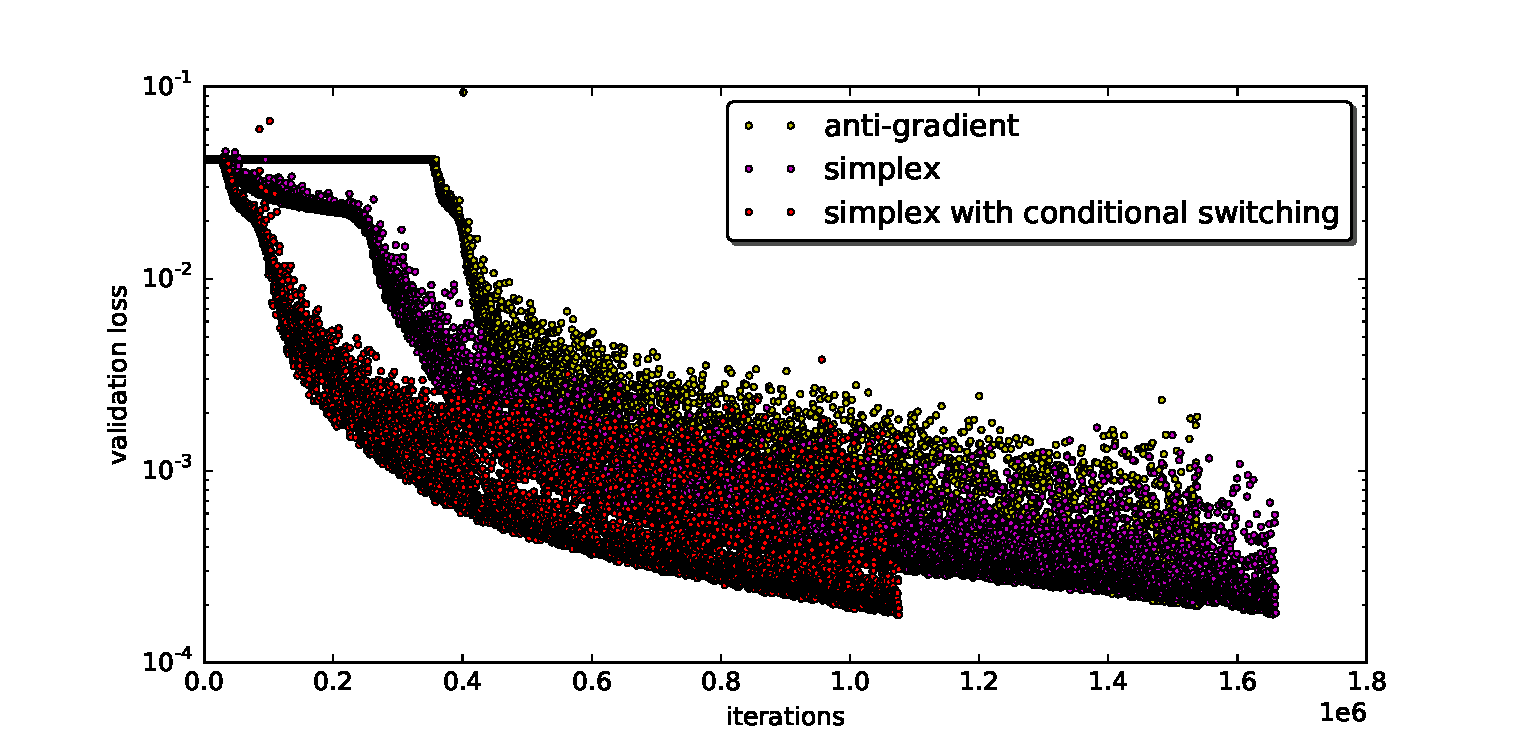
\includegraphics[width= 1\textwidth]{compare_simplex_add_new.eps}\label{fig:compare_add_13}}\\
	     \vspace{0em}
	     \subfloat[][Number of iterations.]{\raisebox{0em}{\resizebox{0.7\columnwidth}{!}{
	     		{\renewcommand{\arraystretch}{1.3}
	     			\setlength{\tabcolsep}{5pt}
	     		\begin{tabular}[b]{C{3cm} | C{3cm} C{5cm}}
	     		& anti-gradient & simplex with conditional switching \\
	     		\hline
	     		addition & 1807466 & \textbf{1630666} \\
	     		temporal order & 	2164800 & \textbf{1010000}\\
	     	\end{tabular}}}
	     }
	    }
%		\caption{Comparison between SGD using as descent direction the anti-gradient, the simplex direction and the simplex direction with conditional switching.}
		\label{fig:1}
	\end{figure}
	
%	\begin{figure}[h]
%		\begin{subfigure}{1.\textwidth}
%			\centering
%			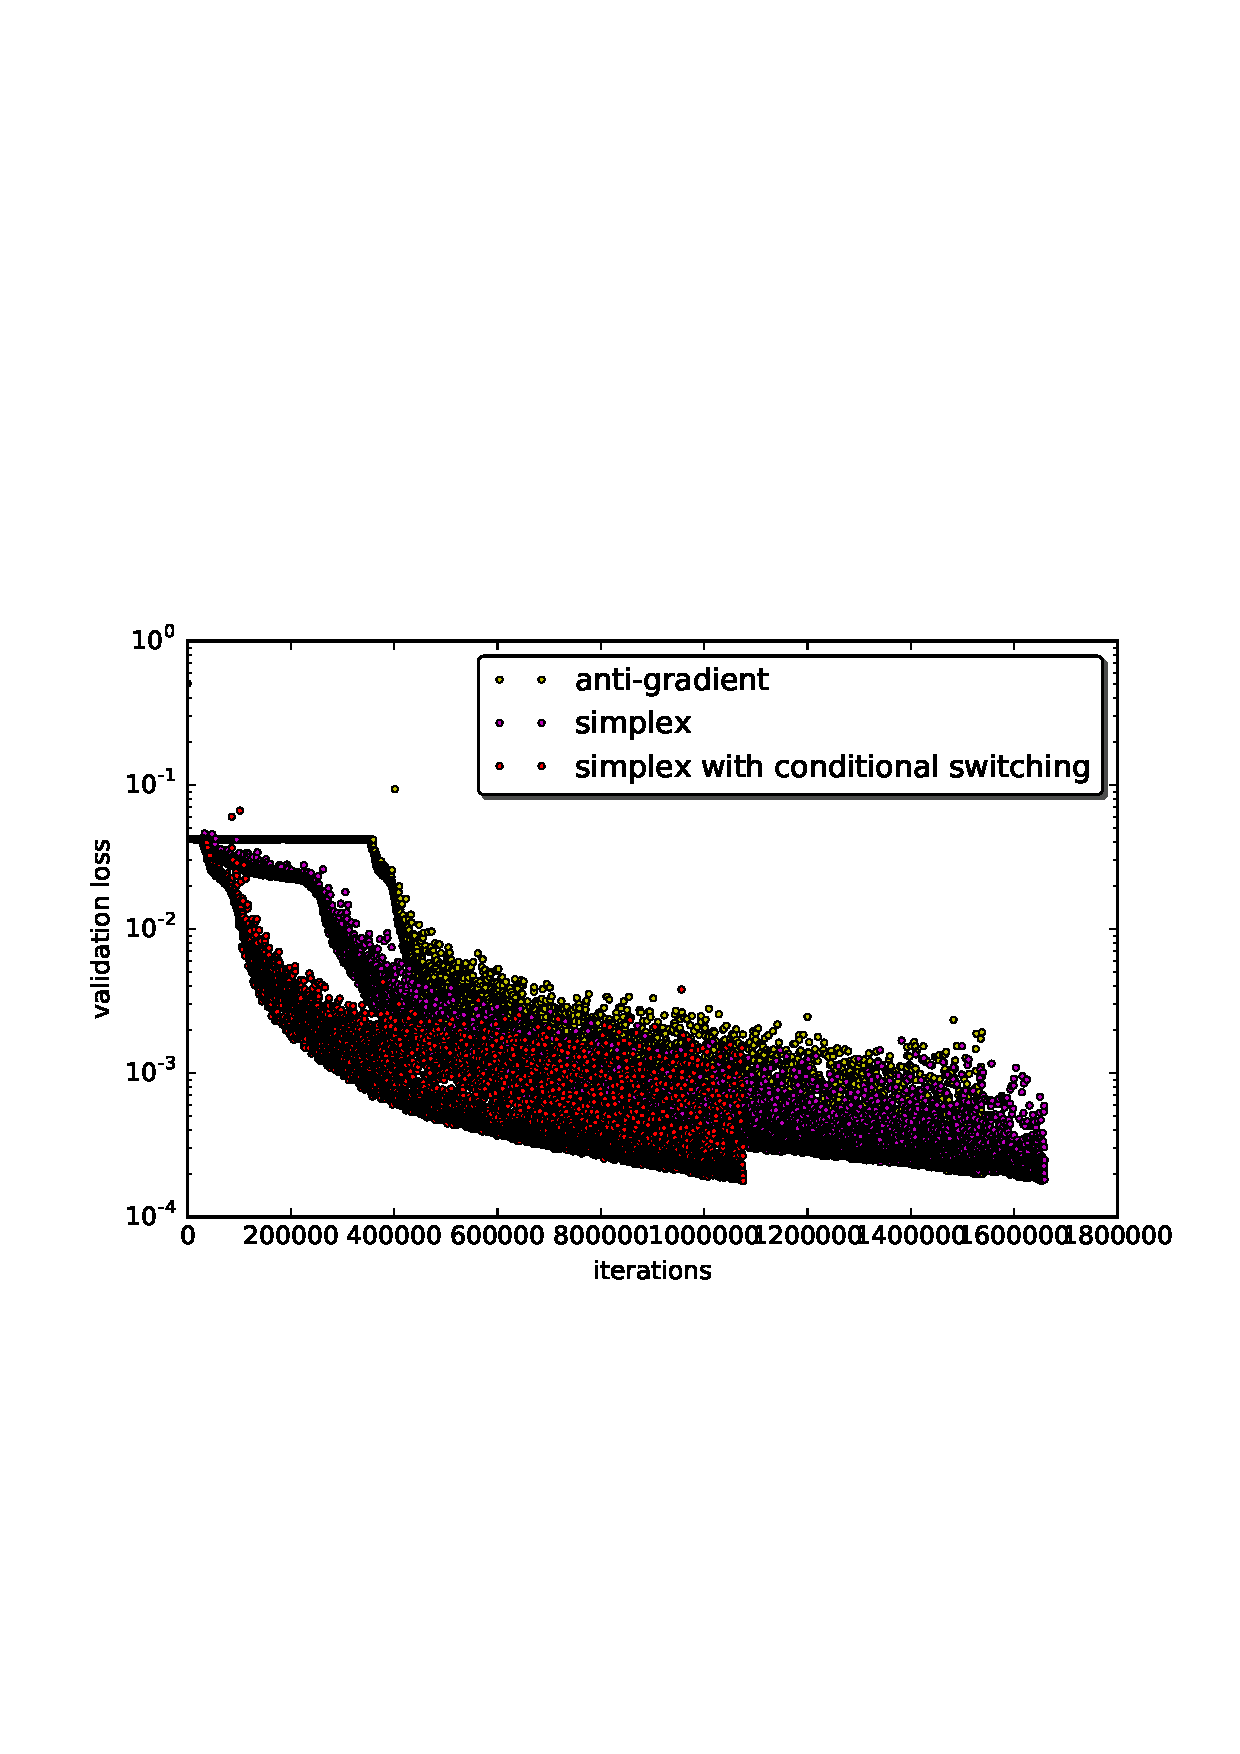
\includegraphics[width= 1\textwidth]{compare_add_simplex_13.png}
%			\caption{First run}
%			\label{fig:a:comparisong_add_simplex}
%		\end{subfigure}\\
%		\begin{subfigure}{1.\textwidth}
%			\centering
%			\includegraphics[width= 1\textwidth]{compare_add_simplex_14.png}
%			\caption{Second run}
%			\label{fig:b:comparisong_add_simplex}
%		\end{subfigure}\\
%		\begin{subfigure}{1.\textwidth}
%			\centering
%			\includegraphics[width= 1\textwidth]{compare_add_simplex_15.png}
%			\caption{Third run}
%			\label{fig:c:comparisong_add_simplex}
%		\end{subfigure}%
%		\caption{Comparison between SGD using as descent direction the anti-gradient (in yellow, start decreasing always for last), the simplex direction (in purple, which is the second that start decreasing) and the simplex direction with conditional switching (in red, start decreasing always for first) for the addition task (T=100). In y axis the loss (mean squared error) in logarithmic scale.}
%		\label{fig:comparisong_add_simplex}
%	\end{figure}
\end{frame}

\section{A real case: Lupus disease prediction}

%\begin{table}
%	\begin{tabular}{ C{1.5cm} | C{0.7cm} C{2cm} C{1.5cm} C{1cm} C{1cm} C{1cm} C{2cm} C{2cm} | C{2cm} }
%		& age & MyasteniaGravis & arthritis & c3level & c4level & hematological & skinrash & sledai2kInferred & SDI \\
%		\hline
%		Visit 0 & 44.23 & 0 & 1 & 119 & 9 & 0 & 0 & 12.0 & 0 \\
%		Visit 1 & 44.63 & 0 & 0 & 96  & 7 & 0 & 0 & 2 & 0 \\
%		Visit 2 & 44.77 & 0 & 1 & 85.42 & 6 & 0 & 0 & 2 & 0 \\
%		Visit 3 & 44.98 & 0 & 1 & 76 & 6 & 0 & 0 & 2 & 0 \\
%		Visit 4:& 45.58 & 0 & 0 & 76 & 6 & 0 & 0 & 1 \\
%	\end{tabular}
%\end{table}

\begin{frame}{Lupus disease prediction}

	The \textbf{goal} is to predict whether a patience will develop the lupus disease in the near future given its medical history.
	\vspace{2em}\\
	Dataset:
	\begin{itemize}
		\item Gathered by the ``Lupus Clinic'', Reumatologia, Università Sapienza, Rome.
		\item Patients have a different number of visits.
		\item Visits are not equally spaced over time.
		\item Small dataset ($\sim100$ negatives, $40$ positives).
	\end{itemize}

\end{frame}

\begin{frame}{An example of a record of a patience}
\begin{table}[H]
	\centering
	\begin{tabular}{ C{2.5cm} | C{1cm} C{1cm} C{1cm} C{1cm} C{1cm}}
		& Visit 0 & Visit 1 & Visit 2 & Visit 3 & Visit 4 \\
		\hline
		age & 44.23 & 44.63 & 44.77 & 44.98 & 45.58 \\
		MyasteniaGravis & 0 & 0 & 0 & 0 & 0 \\
		arthritis & 1 & 0 & 1 & 1 & 0 \\
		c3level & 119 & 96 & 85.42 & 76 & 76 \\
		c4level & 9 & 7 & 6 & 6 & 6 \\
		hematological & 0 & 0 & 6 & 6 & 6 \\
		skinrash & 0 & 0 & 0 & 0 & 0 \\
		sledai2kInferred & 12 & 2 & 2 & 2 & 0 \\
		\dots & \dots & \dots & \dots & \dots & \dots \\
		\hline
		SDI & 0 & 0 & 0 & 0 & \textbf{1}\\
	\end{tabular}
\end{table}	
\end{frame}


\begin{frame}{Numerical results for the lupus disease prediction}

\begin{figure}
	\centering
		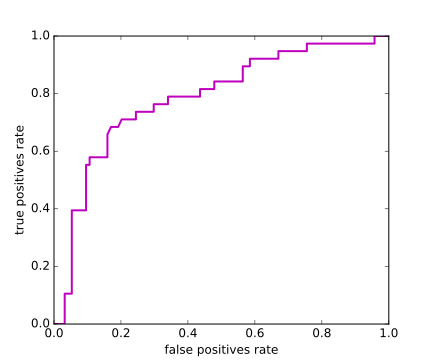
\includegraphics[width= 0.6\textwidth]{plot_roc_lupus_roc_.eps}
		%			\caption{roc curve for models of Line 5 of Table \ref{table:exp_res}.}
		\caption{ROC curve. AUC score is 0.74}
		\label{fig:lupus_roc}
\end{figure}

\begin{itemize}
	\item Results considered promising by medical experts.
	\item Improvable when more data will be available.
\end{itemize}

\end{frame}


 


\section{}
\begin{frame}[allowframebreaks]{References}
	\bibliographystyle{ieee}
	\bibliography{biblio}
\end{frame}

\end{document} 
